\documentclass{article}
\usepackage[utf8]{inputenc}
\usepackage[super,square]{natbib}
\usepackage{tabularx}
\usepackage{parskip}
\usepackage[margin=1.4in]{geometry}
\usepackage{csquotes}
\usepackage{amsmath}
\usepackage{amsfonts}
\usepackage{amsthm}
\usepackage{hyperref}
\usepackage{graphicx}
\usepackage{float}
\usepackage{textcomp}
\usepackage{multicol}
\usepackage{color,soul}

\hypersetup{
    colorlinks,
    citecolor=black,
    filecolor=black,
    linkcolor=black,
    urlcolor=black
}

%%%%%% Begin code snippet config %%%%%% 
\usepackage{listings}
\usepackage{xcolor}
%New colors defined below
\definecolor{codegreen}{rgb}{0,0.6,0}
\definecolor{codegray}{rgb}{0.5,0.5,0.5}
\definecolor{codepurple}{rgb}{0.58,0,0.82}
\definecolor{backcolour}{rgb}{0.95,0.95,0.92}

%Code listing style named "mystyle"
\lstdefinestyle{mystyle}{
  backgroundcolor=\color{backcolour},   commentstyle=\color{codegreen},
  keywordstyle=\color{magenta},
  numberstyle=\tiny\color{codegray},
  stringstyle=\color{codepurple},
  basicstyle=\ttfamily\footnotesize,
  breakatwhitespace=false,         
  breaklines=true,                 
  captionpos=b,                    
  keepspaces=true,                 
  numbers=left,                    
  numbersep=5pt,                  
  showspaces=false,                
  showstringspaces=false,
  showtabs=false,                  
  tabsize=2
}

%"mystyle" code listing set
\lstset{style=mystyle}
%%%%%% End code snippet config %%%%%% 


% Book headers
% \usepackage{fancyhdr}

% \pagestyle{fancy}
% \fancyhf{}
% \fancyhead[L]{\rightmark}
% \fancyhead[R]{\thepage}
% \renewcommand{\headrulewidth}{0pt}


\newcommand{\comment}[1]{}
\newcommand{\bigO}{\mathcal{O}}
\title{\vspace{-3cm} Data Structures and Algorithms}
\author{}
\date{}

\comment{
TODO: 
- Add ML algorithms
    - regression
    - minimax
    - k nearest neighbors
- Add Flow networks to DS
    - Ford fulkerson max-flow algorithm
    - http://www.cs.sjtu.edu.cn/~jiangli/teaching/CS222/files/materials/Algorithm%20Design.pdf
}

\begin{document}
\maketitle
\vspace{-1.5cm}
\tableofcontents
\newpage

\section{Pre-requisite Concepts}

    \subsection{Asymptotic Runtime Analysis}
    \subsubsection{Big O}
    We can measure the growth rate of the time or space complexity of an algorithm using an upper bound ($\bigO(f)$), lower bound ($\Omega (f) $) or a tight bound ($\Theta (f)$) on the best, worst or average case run time. When analysing an algorithm we typically use an upper bound on the worst case. 
    \[
        \bigO(1) \leq \bigO(\log n) \leq \bigO(n) \leq \bigO(n \log n) \leq \bigO(n^2) \leq  \bigO(2^n)  \leq \bigO(n!)
    \]
    \begin{multicols}{2}
    \begin{itemize}
        \item[] $\bigO(1)$ - constant time
        \item[] $\bigO(\log(n))$ - logarithmic time
        \item[] $\bigO((\log(n))^c)$ - polylogarithmic time
        \item[] $\bigO(n)$ - linear time
        \item[] $\bigO(n^2)$ - quadratic time
        \item[] $\bigO(n^c)$ - polynomial time
        \item[] $\bigO(c^n)$ - exponential time
        \item[] $\bigO(n!)$ - factorial time
    \end{itemize}
    \end{multicols}
    
    \subsubsection{Amortized Analysis}
    If the cost of an action has high variance, i.e. its computation is often inexpensive but is occasionally expensive, we can capture its expected behaviour using an amortized time value. If we let $T(n)$ represent the amount of work the algorithm does on an input of size $n$, An operation has amortized cost $T(n)$ if $k$ operations cost $\leq k \cdot T(n)$. $T(n)$ being amortized roughly means $T(n)$ is averaged over all possible operations. 
    
    For example, a dynamic array will copy over elements to an array of double its size whenever an insert is called on an already full instance, otherwise it will simply insert the new element. For $n$ insertions, this happens on every $2, 4, 8, ..., n$ element.
    \[
        T(n) = \bigO ( n + \frac{n}{2} + \frac{n}{4} + \cdots + 1) 
        = \bigO(2n) 
    \]
    Therefore, $n$ insertions take $\bigO(2n)$ time and the amortized time for each insertion is $\bigO(1)$. 
    
    A data structure realizing an amortized complexity of $\bigO (f(n))$ is less performant than one with a worst-case complexity is $\bigO(f(n))$, since a very expensive operation might still occur, but it is better than an algorithm with an average-case complexity $\bigO(f(n))$, since the amortized bound will achieve this average on any input.
    
    \subsubsection{Logarithmic Runtime}
    When encountering an algorithm in which the number of elements in the problem space is halved on each step, i.e. in a divide and conquer solution like binary search, the algorithm will likely have a $\bigO(\log n)$ or $\bigO(n \log n)$ run-time. We can think of $\bigO(n \log n)$ as doing $\log n$ work $n$ times. 
    
    Again, if we let $T(n)$ represent the amount of work the algorithm does on an input of size $n$,
    \begin{align*}
        T(n) &= T(n/2) + \Theta(1) \\
        &=  T(n/4)+ \Theta(1) + \Theta(1) \\ 
        &= \Theta(1) + \cdots + \Theta(1) \\
        &= \Theta(\log n ) 
    \end{align*}
    
    When using Python's standard library sort on an array, we can assume the running time will be $\bigO (n \log n)$. See section on Timsort for further details.
    
    \subsection{Computational Complexity}
    \subsubsection{Complexity Classes}
    \[
        P \subseteq NP \subseteq EXP \subseteq R
    \]
    
    \begin{enumerate}
        \item $P$:  The set of problems that can be solved in polynomial time.
        \item $NP$:  The set of decision problems that can be solved in non-deterministic polynomial time via a ``lucky'' algorithm.
        \item $EXP$: The set of problems that can be solved in exponential time. 
        \item $R$: The set of problems that can be solved in finite time.
    \end{enumerate}
    
    \subsubsection{NP Problems}
    Nondeterminsitic Polynomial (NP) problems follow a nondeterministic model in which an algorithm makes guesses and produce a binary output of YES or NO. These are the simplest interesting class of problems and are known as decision problems. A ``lucky” algorithm can make guesses which are always correct without having to attempt all options. In other words, $NP$ is the set of decision problems with solutions that can be verified in polynomial time. This means that when an answer is YES, it can be proved and a polynomial-time algorithm can verify the proof.
    
    P vs. NP asks whether generating proofs of solutions is harder than checking, i.e whether every problem whose solution can be quickly verified can also be solved quickly. NP-hard problems are those at least as hard as all NP problems. NP-hard problems need not be in NP; that is, they may not have solutions verifiable in polynomial time. NP-complete problems are a set of problems to each of which any other NP-problem can be reduced in polynomial time and whose solution may still be verified in polynomial time. In fact, NP-complete = NP $\cap$ NP-hard.
    
    \subsubsection{Reductions}
    A reduction is an algorithm for transforming one problem into another problem for which a solution or analysis already exists (instead of solving it from scratch). A sufficiently efficient reduction from one problem to another may be used to show that the second problem is at least as difficult as the first. 
    
    NP-complete problems are all interreducible using polynomial-time reductions (same difficulty). This implies that we can use reductions to prove NP-hardness. A one-call reduction is a polynomial time algorithm that constructs an instance of $X$ from an instance $Y$ so that their optimal values are equal, i.e. $X$ problem $\implies$ $Y$ problem $\implies$ $Y$ solution $\implies$ $X$ solution. Multicall reductions instead solve $X$ using free calls to $Y$ -- in this sense, every algorithm reduces the problem and model of computation.
    
    
    \subsection{Algorithm Design}
    \subsubsection{In-place algorithm}
        An in-place algorithm is an algorithm which transforms input using no auxiliary data structure, though a small amount of extra storage space is allowed for a constant number of auxiliary variables. The input is usually overwritten by the output (mutated) as the algorithm executes. An in-place algorithm updates input sequence only through replacement or swapping of elements.
        
    \subsubsection{Space–time tradeoff}
        A space–time or time–memory trade-off is a case where an algorithm trades increased space usage with decreased time complexity. Here, space refers to the data storage consumed in performing a given task (RAM, HDD, etc), and time refers to the time consumed in performing a given task (computation time or response time).
        
    \subsubsection{Heuristics}
        A heuristic is a technique designed for solving a problem more quickly when classic methods are too slow, or for finding an approximate solution when classic methods fail to find any exact solution. This is achieved by trading optimality, completeness, accuracy, or precision for speed. In a way, it can be considered a shortcut.
    
    \subsubsection{Hash Functions}
        A hash function is any function that can be used to map data of arbitrary size to fixed-size values. The values returned by a hash function are called hash values, hash codes, digests, or simply hashes. 
        A good hash function satisfies two basic properties: it should be very fast to compute; it should minimize duplication of output values (\textbf{collisions}). For many use cases, it is useful for every hash value in the output range to be generated with roughly the same probability. Two of the most common hash algorithms are the MD5 (Message-Digest algorithm 5) and the SHA-1 (Secure Hash Algorithm).

    \subsubsection{Stack vs. Heap Memory Allocation}
    The stack is the memory set aside as scratch space for a thread of execution. When a function is called, a block of fixed size is reserved on the top of the stack for local variables and some bookkeeping data. When that function returns, the block becomes freed for future use. The stack is always reserved in a LIFO (last in first out) order; the most recently reserved block is always the next block to be freed. This makes it really simple and fast to keep track of and access the stack; freeing a block from the stack is nothing more than adjusting one pointer. Also, each byte in the stack tends to be reused very frequently which means it tends to be mapped to the processor's cache, making it very fast.

    The heap is memory set aside for dynamic allocation by the OS through the language runtime. Unlike the stack, there's no enforced pattern to the allocation and deallocation of blocks from the heap. The size of the heap is set on application startup, but can grow as space is needed. This makes it much more complex to keep track of and access which parts of the heap are allocated or free at any given time. Another performance hit for the heap is that the heap, being mostly a global resource, typically has to be multi-threading safe.

\newpage
\section{Data Structures and ADTs}
    An \textbf{abstract data type (ADT)} is a theoretical model of an entity and the set of operations that can be performed on that entity
    
    A \textbf{data structure} is a value in a program which can be used to store and operate on data, i.e. it is a programmed implementation of an ADT.
    
    \textbf{Contiguously-allocated structures} are composed of single slabs of memory, and include arrays, matrices, heaps, and hash tables.
     
    \textbf{Linked data structures} are composed of distinct chunks of memory bound together by pointers, and include lists, trees, and graph adjacency lists. Recall, a pointer is a reference to a memory address which stores some data.

    \subsection{Lists and Arrays}
    \subsubsection{List}
    A list is an abstract data type that represents a countable number of ordered values, where the same value may occur more than once. Lists are a basic example of containers, as they contain other values. Their operations include the following,
    \begin{itemize}
        \item \textbf{isEmpty(L)}: test whether or not the list is empty
        \item \textbf{prepend(L, item)}: prepend an entity to the list
        \item \textbf{append(L, item)}: append an entity to the list
        \item \textbf{get(L, i)}: access the element at a given index.
        \item \textbf{head(L)}: determine the first component of the list
        \item \textbf{tail(L)}: refer to the list consisting of all the components of a list except for its first (head).
    \end{itemize}
    
    \subsubsection{Arrays}
    An array is a data structure implementing a list ADT, consisting of a collection of elements (values or variables), each identified by at least one array index or key. 
    
    A \textbf{bit array} (a.k.a bit map) is a data structure which uses an array of 0's and 1's to compactly store information. An index $j$ with a value of 1 indicates the presence of an integer corresponding to $j \in \mathbb Z$. When given a constraint on possible values that need to be stored and analyzed, we can initialize a bit array with a size of the max possible value and record frequencies directly in their corresponding index, eliminating the need to re-order an unsorted array or maintain a sorted order on every insertion. We can extend the bit array to store arbitrary integers, i.e. an int of value 3 in index 10 may indicate we've encountered 3 values of 10. 
    
    
    A \textbf{dynamic array} is a data structure that allocates all elements contiguously in memory and keeps a count of the current number of elements. If the space reserved for the dynamic array is exceeded, it is reallocated and (possibly) copied, which is an expensive operation. Though its amortized insertion cost is equal to a static array, $\Theta(1)$. Python's  ``List'' data structure is a dynamic array which uses table doubling to support its constant amortized operations. It is possible to implement real-time table doubling to support constant worst-caseRa insertions by incrementally building up a larger array by some to quickly switch to when the original array is full.
    
    \vspace{8pt} \emph{Time Complexity of List operations}
    \begin{table}[H]
        % \centering
        \begin{tabular}{|l|l|l|}
            \hline
            \textbf{Operation} & \textbf{Average Case} & \textbf{Amortized Worst Case} \\
            \hline
            Copy & $\bigO(n)$ & $\bigO(n)$ \\
            Append & $\bigO(1)$ & $\bigO(1)$\\
            Pop last & $\bigO(1)$ & $\bigO(1)$ \\
            Pop intermediate & $\bigO(k)$ & $\bigO(k)$ \\
            Insert & $\bigO(n)$ & $\bigO(n)$ \\
            Get Item & $\bigO(1)$ & $\bigO(1)$ \\
            Set Item & $\bigO(1)$ & $\bigO(1)$ \\
            Delete Item & $\bigO(n)$ & $\bigO(n)$ \\
            Iteration & $\bigO(n)$ & $\bigO(n)$ \\
            Get Slice & $\bigO(k)$ & $\bigO(k)$\\
            Del Slice & $\bigO(n)$ & $\bigO(n)$ \\
            Set Slice & $\bigO(k+n)$ & $\bigO(k+n)$\\
            Extend & $\bigO(k)$ & $\bigO(k)$\\
            Sort & $\bigO(n\log n)$ &$\bigO(n\log n)$\\
            Multiply & $\bigO(nk)$ & $\bigO(nk)$ \\
            x in s & $\bigO(n)$ &  \\
            min(s), max(s) & $\bigO(n)$ & \\
            Get Length & $\bigO(1)$ & $\bigO(1)$ \\
            \hline
        \end{tabular}
    \end{table}

    
    \subsubsection{Linked Lists}
    A linked list is a data structure that represents a sequence of nodes. In a singly linked list each node maintains a pointer to the next node in the linked list. A doubly linked list gives each node pointers to both the next node and the previous node. Unlike an array, a linked list does not provide constant time access to a particular ``index'' within the list, i.e. to access the $K$th index you will need to iterate through $K$ elements. The benefit of a linked list is that inserting and removing items from the beginning of the list can be done in constant time. For specific applications, this can be useful. Linked structures can have poor cache performance compared with arrays. Maintaining a sorted linked list is costly and not usually worthwhile since we cannot perform binary searches.

    
\vspace{8pt} \emph{Python Implementation}
\begin{lstlisting}[language=Python]
class ListNode:
    def __init__(self, val=0, next=None):
        self.val = val
        self.next = next
\end{lstlisting}
        
    \subsubsection{Self-Organizing Lists}
    A self-organizing list is a list that reorders its elements based on some self-organizing heuristic to improve average access time. The aim of a self-organizing list is to improve efficiency of linear search by moving more frequently accessed items towards the head of the list. A self-organizing list achieves near constant time for element access in the best case and uses a reorganizing algorithm to adapt to various query distributions at runtime.
    
    \subsubsection{Skip Lists}
    As an alternative to balanced trees examined later, a hierarchy of sorted linked lists is maintained, where a random variable is associated to each element to decide whether it gets copied into the next highest list. This implies roughly $\log n$ lists, each roughly half as large as the one above it. A search starts in the smallest list. The search key lies in an interval between two elements, which is then explored in the next larger list. Each searched interval contains an expected constant number of elements per list, for a total expected $\bigO(\log n)$ query time. The primary benefits of skip lists are ease of analysis and implementation relative to balanced trees.
    
    \subsection{Stacks and Queues}
    \subsubsection{Stacks}
    A stack is an ADT container that uses last-in first-out (LIFO) ordering, i.e. the most recent item added to the stack is the first item to be removed. It supports the following operations:
    \begin{itemize}
        \item  \textbf{pop()}: Remove the top item from the stack.
        \item  \textbf{push(item)}: Add an item to the top of the stack.
        \item \textbf{peek()}: Return the top of the stack.
        \item \textbf{isEmpty()}: Return true if and only if the stack is empty.
    \end{itemize}
    Unlike an array, a stack does not offer constant-time access to the $i$th item. However, it does allow constant time adds and removes as it doesn't require shifting elements around. One case where stacks are often useful is in certain recursive algorithms where we need to push temporary data onto a stack as we recurse and then remove them as we backtrack (for example, because the recursive check failed). A stack offers an intuitive way to do this. A stack can also be used to implement a recursive algorithm iteratively which is what's otherwise done in a functions call stack.
    
    \subsubsection{Queues}
    A queue is an ADT container that implements FIFO (first-in first-out) ordering, i.e. items are removed in the same order that they are added. It supports the following operations: 
    \begin{itemize}
        \item \textbf{push(item)}: Add an item to the end of the queue.
        \item \textbf{popLeft()}: Remove and return the first item in the queue.
        \item \textbf{peek()}: Return the top of the queue.
        \item \textbf{isEmpty()}: Return true if the queue is empty. 
    \end{itemize}
    
    One place where queues are often used is in breadth-first search or in implementing a cache. In breadth-first search we may use a queue to store a list of the nodes that we need to process. Each time we process a node, we add its adjacent nodes to the back of the queue. This allows us to process nodes in the order in which they are viewed. 
    
    A queue can be implemented with a linked list and moreover, they are essentially the same thing as long as items are added and removed from opposite sides.
    
    The deque module (short for double-ended queue), provides a data structure which pops from or pushes to either side of the queue with the same $\bigO(1)$ performance. 
    
\vspace{8pt} \emph{Python Implementation}
\begin{lstlisting}[language=Python]
from collections import deque 

q = deque() 
for item in data:
    q.append(item) 
 
while len(q):
    next_item = q.popleft() # array.pop(0)
    print(next_item)

\end{lstlisting}

    \vspace{8pt} \emph{Time Complexity of collections.deque operations}
    \begin{table}[H]
        % \centering
        \begin{tabular}{|l|l|l|}
            \hline
            \textbf{Operation} & \textbf{Average Case} & \textbf{Amortized Worst Case} \\
            \hline
            Copy & $\bigO(n)$ & $\bigO(n)$ \\
            append & $\bigO(1)$ & $O(1)$ \\
            appendleft & $\bigO(1)$ & $\bigO(1)$ \\
            pop & $\bigO(1)$ & $\bigO(1)$ \\
            popleft & $\bigO(1)$ & $\bigO(1)$ \\
            extend & $\bigO(k)$ & $\bigO(k)$ \\
            extendleft & $\bigO(k)$ & $\bigO(k)$ \\
            rotate & $\bigO(k)$ & $\bigO(k)$\\
            remove & $\bigO(n)$ & $\bigO(n)$\\
            \hline
        \end{tabular}
    \end{table}

    
    \subsubsection{Priority Queue}
    A priority queue is an ADT container that retrieves items not by the insertion time (as in a stack or queue), nor by a key match (as in a dictionary), but instead retrieves items with the highest priority value. Priority queues provide more flexibility than simple sorting because they allow new elements to enter a system at arbitrary intervals. It is much more cost-effective to insert a new job into a priority queue than to re-sort everything on each arrival. Max-priority queues order values in descending order with higher priority first and are typically implemented with a max-heap. Min-priority queues sort values in ascending order with lower priority values first and are typically implemented with a min-heap.
    
    The basic priority queue supports three primary operations:
    \begin{itemize}
        \item \textbf{insert(Q, x)}: Given an item x with key k, insert it into the priority queue Q.
        \item \textbf{findMinimum(Q)} or \textbf{findMaximum(Q)}: Return a pointer to the item whose key value is smaller (larger) than any other key in the priority queue Q.
        \item \textbf{deleteMinimum(Q)} or \textbf{deleteMaximum(Q)}: Remove the item from the priority queue Q whose key is minimum (maximum).
    \end{itemize}

    There are several choices in which underlying data structures can be used for a basic priority queue implementation:
    \begin{enumerate}
        \item Binary heaps are the right answer when the upper bound on the number of items in your priority queue is known, since you must specify array size at creation time. Though this constraint can be mitigated by using dynamic arrays
    
        \item Binary search trees make effective priority queues, since the smallest element is always the leftmost leaf, while the largest element is always the rightmost leaf. The min (max) is found by simply tracing down left (right) pointers until the next pointer is nil. Binary tree heaps prove most appropriate when you need other dictionary operations, or if you have an unbounded key range and do not know the maximum priority queue size in advance.
        
        \item Sorted arrays are very efficient in both identifying the smallest element and deleting it by decrementing the top index. However, maintaining the total order makes inserting new elements slow. Sorted arrays are only suitable when there will be few insertions into the priority queue.
        
        \item Bounded height priority queue
        
        \item Fibonacci and pairing heaps. These complicated priority queues are designed to speed up decrease-key operations, where the priority of an item already in the priority queue is reduced. This arises, for example, in shortest path computations when we discover a shorter route to a vertex v than previously established.
    \end{enumerate}
    
    Note: The Queue.PriorityQueue module is a partial wrapper around the heapq module. Max priority queues can be created by inverting priority values before insertion. See binary heap section for more details about heapq.
    
\vspace{8pt} \emph{Python Implementation}
\begin{lstlisting}[language=Python]
# The queue module for a min-priority queue
from queue import PriorityQueue

pq = PriorityQueue()
for item in data:
    pq.put((item.priority, item))

while not pq.empty():
    next_item = pq.get()
    print(next_item)
    
# The heapq module for a min-priority queue
import heapq
pq = []
for entry_count, item in enumerate(data):
    heapq.heappush(pq, (item.priority, entry_count, item))
    
while pq:
    next_item = heapq.heappop(pq)
    print(next_item)
\end{lstlisting}

    \subsubsection{Indexed Priority Queue}
    An Indexed Priority Queue gives us the ability to change the priority of an element without having to go through all the elements. It can be thought of as a combination of a hash table, used for quick lookups of values, and a priority queue, to maintain a heap ordering.

    \subsubsection{Monotonic Stack and Queue}
    This structure maintains an ordering so that its elements are either strictly increasing or strictly decreasing. It differs from a heap in that instead of re-ordering elements as they're processed, it will discard previous numbers that do not follow the monotonic condition before appending a new number. 
    
    A monotonic decreasing stack can be useful for finding the index distance of the next smaller number given an unordered list of numbers. Instead of searching for the next smallest number for every number, resulting in an $\bigO(n^2)$ runtime, we only need to check the top of the stack of indicies of previously visited numbers, giving us a $\bigO(n)$ runtime. 
    
    In some application we might also need to remove elements from the front and back, thus a double-ended queue (deque from collections module) should be used. In an increasing queue, we find the first element smaller than current, either in the left (from pushing in) or in the right (from popping out). In a decreasing queue we find the first element larger than current, either in the left (from pushing in) or in the right (from popping out). A monotonic queue can also useful for implementing a variant of the sliding window. See sliding window section for an example.
    
\vspace{8pt} \emph{Python Implementation}
\begin{lstlisting}[language=Python]
def monotonic_stack(A):
    smaller_to_right = [-1] * len(A)
    stack = []
    for i, v in enumerate(A):
        while stack and A[stack[-1]] < v:
            cur = stack.pop()
            smaller_to_right[cur] = i - cur
        stack.append(i)
    return smaller_to_right

import collections
def monotonic_deque(A):
    dq = collections.deque()
    smaller_to_left, smaller_to_right = [-1] * len(A), [-1] * len(A)
    for i, v in enumerate(A):
        while dq and A[dq[-1]] >= v: 
            smaller_to_right[dq.pop()] = v 
        if dq:  
            smaller_to_left[i] = A[dq[-1]]
        dq.append(i)
    return smaller_to_left, smaller_to_right
\end{lstlisting}

    \subsection{Hash Tables}
    A hash table is a data structure that maps keys to values for highly efficient lookup. There are a number of ways of implementing this, but a simple but common implementation is known as \textbf{separate chaining}. In this implementation, we use an array of linked lists and a hash code function. To insert a key (which might be a string or essentially any other data type) and value, we do the following: 
    \begin{enumerate}
        \item 
        First, compute the key's hash code, which will usually be an \textit{int} or \textit{long}. Note that two different keys could have the same hash code, as there may be an infinite number of keys and a finite number of hash codes.
        \item
        Then, map the hash code to an index in the array. This could be done with something like $hash(key)\mod array\_length$. Two different hash codes could map to the same index.
        \item
        At this index, there is a linked list of keys and values. Store the key and value in this index. We must use a linked list because of collisions: you could have two different keys with the same hash code, or two different hash codes that map to the same index.
    \end{enumerate}
    To retrieve the value pair by its key, you repeat this process. Compute the hash code from the key, and then compute the index from the hash code. Then, search through the linked list for the value with this key. If the number of collisions is very high, the worst case runtime is $\bigO(n)$, where $n$ is the number of keys. However, we generally assume a good implementation that keeps collisions to a minimum, in which case the lookup time is $\bigO(1)$. Alternatively, we can implement the hash table with a balanced binary search tree. This gives us an $\bigO(\log n)$ lookup time. The advantage of this is potentially using less space, since we no longer allocate a large array. We can also iterate through the keys in order, which can be useful sometimes.

    The other strategy used to resolve collisions is to require each array element to contain only one key, but to also allow keys to be mapped to alternate indices when their original spot is already occupied. This is known as \textbf{open addressing}. In this type of hashing, we have a parameterized hash function $h$ that takes two arguments, a key and a positive integer. Searching or \textbf{probing} for an item requires examining not just one spot, but many spots until either we find the key, or reach a None value. After we delete an item, we replace it with a special value Deleted, rather than simply None. This way, the Search algorithm will not halt when it reaches an index that belonged to a deleted key.
    
    The simplest implementation of open addressing is \textbf{linear probing}: start at a given hash value and then keep adding some fixed offset to the index until an empty spot is found. The main problem with linear probing is that the hash values in the middle of a cluster will follow the exact same search pattern as a hash value at the beginning of the cluster. As such, more and more keys are absorbed into this long search pattern as clusters grow. We can solve this problem using \textbf{quadratic probing}, which causes the offset between consecutive indices in the probe sequence to increase as the probe sequence is visited. \textbf{Double hashing} resolves the problem of a form of clustering occurs where if many items have the same initial hash value, they still follow the exact same probe sequence. It does this by using a hash function for both the initial value and its offset.

    A useful hash function for strings is,
    \[
        H(S,j) = \sum_{i=0}^{m-1} \alpha^{m-(i+1)} \cdot char(s_{i+j}) \mod m
    \]
    where $\alpha$ is the size of the alphabet and $char(x)$ is the ASCII character code. This hash function has the useful property allowing hashes of successive m-character windows of a string to be computed in constant time instead of $\bigO(m)$.
    \[
        H(S, j+1) = (H(S,j) - \alpha^{m-1}char(s_j))\alpha + s_{j+m}
    \]
    
    \subsubsection{Dictionaries}
    The dictionary data type (a.k.a. hash table or hash map) permits access to data items based on its content. You insert an item into a dictionary so you can retrieve it when you need it.
    
    Python dicts use open addressing to resolve hash collisions which uses random probing in which the next slot is picked in a pseudo random order. The entry is then added to the first empty slot.
    
    The primary operations a dictionary supports are:
    \begin{itemize}
        \item  \textbf{search(D, k)} – Given a search key $k$, return a pointer to the element in dictionary $D$ whose key value is $k$, if one exists.
        \item \textbf{insert(D, x)} – Given a data item $x$, add it to the set in the dictionary $D$.
        \item \textbf{delete(D, x)} – Given a pointer to a given data item $x$ in the dictionary $D$, remove it from $D$.
        \item \textbf{max(D)} or \textbf{min(D)} – Retrieve the item with the largest (or smallest) key from $D$. This enables the dictionary to serve as a priority queue.
        \item \textbf{predecessor(D, k)} or \textbf{successor(D, k)} – Retrieve the item from $D$ whose key is immediately before (or after) $k$ in sorted order. These enable us to iterate through the elements of the data structure.
    \end{itemize}
    
   \vspace{8pt} \emph{Time Complexity of dict Operations}
    \begin{table}[H]
        % \centering
        \begin{tabular}{|l|l|l|}
            \hline
            \textbf{Operation} & \textbf{Average Case} & \textbf{Amortized Worst Case} \\
            \hline
            k in d & $\bigO(1)$ & $\bigO(n)$ \\
            Copy & $\bigO(n)$ & $\bigO(n)$ \\
            Get Item & $\bigO(1)$ & $\bigO(n)$ \\
            Set Item & $\bigO(1)$ & $\bigO(n)$ \\
            Delete Item & $\bigO(1)$ & $\bigO(n)$ \\
            Iteration & $\bigO(n)$ & $\bigO(n)$ \\
            \hline
        \end{tabular}
    \end{table}
    
    \subsubsection{Sets}
    In mathematical terms, a set is an unordered collection of unique objects drawn from a fixed universal set. A hash set implements the set ADT using a hash table. Sorted order turns the problem of finding the union or intersection of two subsets into a linear-time operation, just sweep from left to right and see what you are missing. It makes possible element searching in sublinear time. Finally, printing the elements of a set in a canonical order paradoxically reminds us that order really doesn’t matter.
     
    If each subset contains exactly two elements, they can be thought of as edges in a graph whose vertices represent the universal set. A system of subsets with no restrictions on the cardinality of its members is called a hypergraph.
    
    \begin{enumerate}
        \item Test whether $u_i \in S_j$
        \item Compute the union or intersection of $S_i$ and $S_j$
        \item Insert or delete members of $S$
    \end{enumerate}
    
    Although sets are commonly implemented with hash tables, other data structures that can be used:
    
    \begin{enumerate}
        \item Containers or dictionaries – A subset can also be represented using a linked list, array, or dictionary containing exactly the elements in the subset.
        \item Bit vectors – An n-bit vector or array can represent any subset $S$ on a universal set $U$ containing $n$ items. Bit $i$ will be 1 if $i \in S$, and $0$ if not.
        \item Bloom filters – We can emulate a bit vector in the absence of a fixed universal set by hashing each subset element to an integer from $0$ to $n$ and setting the corresponding bit.
    \end{enumerate}
    
    \vspace{8pt} \emph{Time Complexity of set operations}
    \begin{table}[H]
        % \centering
        \begin{tabular}{|l|l|l|}
            \hline
            \textbf{Operation} & \textbf{Average Case} & \textbf{Amortized Worst Case} \\
            \hline
            x in s & $\bigO(1)$ & $\bigO(n)$ \\
            Union & $\bigO(len(s)+len(t))$  & \\
            Intersection & $\bigO(min(len(s), len(t))$ & $\bigO(len(s) * len(t))$ \\
            Multiple intersection & $\bigO(n-1)*\bigO(max(len(s_i)))$ &\\
            Difference & $\bigO(len(s))$ & \\
            Difference Update & $\bigO(len(t))$ & \\
            Symmetric Difference & $\bigO(len(s))$ & $\bigO(len(s) * len(t))$ \\
            Symmetric Difference Update & $\bigO(len(t))$ & $\bigO(len(t) * len(s))$\\
            \hline
        \end{tabular}
    \end{table}

    \subsection{Trees}
    A tree is an ADT composed of nodes such that there is a root node with zero or more child nodes where each child node also has zero or more child nodes and can be recursively defined as a root node of a sub-tree. Since there are no edges between sibling nodes, a tree cannot contain cycles. Furthermore, nodes can be given a particular order, can have any data type as values, and they may or may not have links back to their parent nodes.
    
    \subsubsection{Binary Trees}
    A binary tree is a tree in which each node has up to two children. 
    
    A \textbf{binary search tree} is a binary tree in which every node $n$ follows a specific ordering property: all left descendants $\leq n <$ all right descendants. An inorder traversal (Left-Node-Right) of a binary search tree will always result in a monotonically increasingly ordered sequence.
    
    A \textbf{complete} binary tree is a binary tree in which every level of the tree is filled, except for perhaps the last level and all of the nodes in the bottom level are as far to the left as possible. A complete tree with $n$ nodes has $\lceil \log n \rceil$ height. There is no ambiguity about where the ``empty'' spots in a complete tree are so we do not need to use up space to store references between nodes, as we do in a standard binary tree implementation. This means that we can store its nodes inside an zero-indexed array. For a node corresponding to index $i$, its left child is stored at index $2i + 1$, and its right child is stored at index $2i + 2$. Going backwards, we can also deduce that the parent of index $i$ (when $i > 0$) is stored at index $\lfloor (i-1)/2 \rfloor$.
    
    A \textbf{full} binary tree is a binary tree in which every node has either zero or two children. A \textbf{perfect} binary tree is one that is both full and complete. A full binary tree with $n$ leaves has $n - 1$ internal nodes. Then the number of unique rooted full binary tree with $n + 1$ leaf nodes, equivalently $n$ internal node, can be counted using the $nth$ Catalan number, $C_n$. View section on Catalan numbers for more details.

\vspace{8pt} \emph{Python Implementation}
\begin{lstlisting}[language=Python]
# n-ary tree using dictionary
from collections import defaultdict

## a tree is a dict whose default values are trees. 
tree = lambda: defaultdict(tree)

# Object-oriented binary tree
class TreeNode:
    def __init__(self, val=0, left=None, right=None):
        self.val = val
        self.left = left
        self.right = right
\end{lstlisting}
    
    \subsubsection{Binary Heaps}
    The \textbf{heap property} states that the key stored in each node is either greater than or equal to or less than or equal to the keys in the node's children, according to some total order. A \textbf{min-heap} is a complete binary tree (filled other than the rightmost elements on the last level) where each node is smaller than its children. The root, therefore, is the minimum element in the tree. The converse holds for a \textbf{max-heap}. We have two key operations on a heap: 
    
    \begin{itemize}
        \item \textbf{insert(x)}: When we insert into a min-heap, we always start by inserting the element at the bottom. We insert at the rightmost spot so as to maintain the complete tree property. Then, we maintain the heap property by swapping the new element with its parent until we find an appropriate spot for the element. We essentially bubble up the minimum element. This takes $\bigO (\log n)$ time, where $n$ is the number of nodes in the heap. 
        
        \item \textbf{findMin()} or \textbf{findMax()}: Finding the minimum element of a min-heap is inexpensive since it will always be at the top. The challenging part is how to remove it while maintaining the heap property. First, we remove the minimum element and swap it with the last element in the heap (the bottommost, rightmost element). Then, we bubble down this element, swapping it with one of its children until the heap property is restored. This algorithm will also take $\bigO( \log n)$ time. 
    \end{itemize}
    
    A heap will be better at findMin/findMax ($\bigO(1)$), while a BST is performant at all finds ($\bigO(\log n)$). A heap is especially good at basic ordering and keeping track of max and mins.
    
    Note, heapq creates a min-heap by default. To create a max-heap, you will need to invert values before storing and after retrieving them. Alternatively, you can define a class to wrap the module and override and invert the comparison method.

\vspace{8pt} \emph{Python Implementation}
\begin{lstlisting}[language=Python]
# Using heapq module
import heapq

items = [1, 6, 4, 2, 5, 7, 3, 9, 8, 10]    

## Min-heap
min_heap = []
for item in items:
    heapq.heappush(min_heap, item)

in_place = items.copy()
heapq.heapify(in_place)
heapq.nsmallest(3, in_place)
while in_place:
    min_item = heapq.heappop(in_place) 
    print(min_item)

## Max-heap
max_heap = []
for item in items:
    heapq.heappush(max_heap, -item)

while max_heap:
    max_item = -heapq.heappop(max_heap) 
    print(max_item)
    
in_place = items.copy()
heapq._heapify_max(in_place)
heapq.nlargest(3, in_place)
while in_place:
    max_item = heapq._heappop_max(in_place)
    print(max_item)

# Max heap full implementation
class MaxHeap:
    def __init__(self, items=[]):
        self.heap = [0]
        for i in items:
            self.heap.append(i)
            self.__floatUp(len(self.heap) - 1)

    def push(self, data):
        self.heap.append(data)
        self.__floatUp(len(self.heap) - 1)

    def peek(self):
        if self.heap[1]:
            return self.heap[1]
        else:
            return False

    def pop(self):
        if len(self.heap) > 2:
            self.__swap(1, len(self.heap) - 1)
            maxVal = self.heap.pop()
            self.__bubbleDown(1)
        elif len(self.heap) == 2:
            maxVal = self.heap.pop()
        else:
            maxVal = False
        return maxVal

    def __swap(self, i, j):
        self.heap[i], self.heap[j] = self.heap[j], self.heap[i]

    def __floatUp(self, index):
        parent = index//2
        if index <= 1:
            return
        elif self.heap[index] > self.heap[parent]:
            self.__swap(index, parent)
            self.__floatUp(parent)

    def __bubbleDown(self, index):
        left = index * 2
        right = index * 2 + 1
        largest = index
        if len(self.heap) > left and self.heap[largest] < self.heap[left]:
            largest = left
        if len(self.heap) > right and self.heap[largest] < self.heap[right]:
            largest = right
        if largest != index:
            self.__swap(index, largest)
            self.__bubbleDown(largest)
\end{lstlisting}

\vspace{8pt} \emph{Time Complexity of heapq operations}
    \begin{table}[H]
        % \centering
        \begin{tabular}{|l|l|l|}
            \hline
            \textbf{Operation} & \textbf{Average Case} & \textbf{Amortized Worst Case} \\
            \hline
            heapify & $\bigO(n)$ & $\bigO(n)$ \\
            heappush & $\bigO(1)$ & $O(\log n)$ \\
            heappop & $\bigO(\log n)$ & $O(\log n)$ \\
            peek & $\bigO(1)$ & $\bigO(1)$\\
            heappushpop & TBD & TBD \\
            heapreplace & TBD & TBD \\
            nlargest & TBD & TBD \\
            nsmallest & TBD & TBD\\
            \hline
        \end{tabular}
    \end{table}


    \subsubsection{Tries (Prefix Trees)}
    A trie is a variant of an n-ary tree in which alphanumeric characters are stored at each node. Each path down the tree may represent a word. The * nodes (sometimes called ``null nodes") are often used to indicate complete words. The actual implementation of these * nodes might be a special type of child (i.e. a TerminatingTrieNode class which inherits from TrieNode) or we can use a boolean flag. A node in a trie could have anywhere from 1 through size of alphabet + 1 children (or, 0 through size of alphabet if a boolean flag is used instead of a * node). 
    
    The complexity of creating a trie is $\bigO(|W| L)$, where $W$ is the number of words, and $L$ is an average length of the word: you need to perform $L$ lookups on average for each of the $W$ words in the set. Same goes for looking up words later: you perform $L$ steps for each of the $W$ words.
    
    Very commonly, a trie is used to store the entire English language for quick prefix lookups. A trie can check if a string is a valid prefix in $\bigO(K)$ time, where $K$ is the length of the string. Many problems involving lists of valid words leverage a trie as an optimization. 
    
    To get autocomplete suggestions, it helps to store the cumulative word along with the end indicator. We can then search the trie up to the prefix end and perform a recursive DFS to find all word end points while appending the results to an array of suggestions. To handle misspellings, a function considers four types of edits: a deletion (remove one letter), a transposition (swap two adjacent letters), a replacement (change one letter to another) or an insertion (add a letter). The edit function returns a list of words within a max $N$ edits from the specified word that exist in a dictionary of known words. We can then find suggestions with DFS as before.
    
    Note, most methods in the trie follow a similar traversal pattern, create a pointer to the root of the tree, iterate over characters of a given word, check if the character is not in the current pointers children and then move the pointer forward to the corresponding child.
    
\vspace{8pt} \emph{Python Implementation}
\begin{lstlisting}[language=Python]
# Trie node as lambda function
import collections
TrieNode = lambda: collections.defaultdict(Trie)

# Trie node as class with end of word attribute
class TrieNode:
    def __init__(self):
        self.word = False
        self.children = {}
        
# Trie dict with end of word indicated by special character
class Trie:
    def __init__(self):
        self.root = {}

    def insert(self, word):
        node = self.root
        for char in word:
            if char not in node:
                node[char] = {}
            node = node[char]
        node['$'] = word

    def search(self, word):
        node = self.root
        for char in word:
            if char not in node:
                return False
            node = node[char]
        return '$' in node

    def startsWith(self, prefix):
        node = self.root
        for char in prefix:
            if char not in node:
                return False
            node = node[char]
        return True
\end{lstlisting}

    \subsubsection{Suffix Trees/Arrays}
    A special kind of trie, called a suffix tree, can be used to index all suffixes in a text in order to carry out fast full text searches. The construction of such a tree for the string $S$ takes linear time and space relative to the length of $S$. A suffix tree is basically like a search trie: there is a root node, edges going out of it leading to new nodes, and further edges going out of those, and so forth. Unlike in a search trie, the edge labels are not single characters. Instead, each edge is labeled using a pair of integers: [from, to], which are pointers into the text. In this sense, each edge carries a string label of arbitrary length, but takes only $\bigO(1)$ space (two pointers).
    
    Some example use cases are as follows:
    \begin{itemize}
        \item Find all occurrences of $q$ as a substring of $S$: In collapsed suffix trees, it takes $\bigO(|q| + k)$ time to find the $k$ occurrences of $q$ in $S$.
        \item Locating a substring if a certain number of mistakes or edits are allowed
        \item Locating matches for a regular expression pattern
        \item Finding Longest common substring to a set of strings in linear-time
        \item Find the longest palindrome in $S$
    \end{itemize}
    
    Storing a string's suffix tree typically requires significantly more space than storing the string itself. Observe that most of the nodes in a trie-based suffix tree occur on simple paths between branch nodes in the tree. Each of these simple paths corresponds to a substring of the original string. By storing the original string in an array and collapsing each such path into a single edge, we have all the information of the full suffix tree in only $\bigO(n)$ space. The label for each edge is described by the starting and ending array indices representing the substring. 
    
    The suffix tree for the string $S$ of length $n$ is defined as a tree such that:
    \begin{enumerate}
        \item The tree has exactly $n$ leaves numbered from $1$ to $n$.
        \item Except for the root, every internal node has at least two children.
        \item Each edge is labelled with a non-empty substring of $S$.
        \item No two edges starting out of a node can have string-labels beginning with the same character.
        \item The string obtained by concatenating all the string-labels found on the path from the root to leaf $i$ spells out suffix $S[i \cdots n]$, for $i$ from $1$ to $n$.
    \end{enumerate}
    Suffix arrays do most of what suffix trees do, while using roughly four times less memory. They are also easier to implement. A suffix array is, in principle, just an array that contains all the $n$ suffixes of $S$ in sorted order. Thus a binary search of this array for string $q$ suffices to locate the prefix of a suffix that matches $q$, permitting an efficient substring search in $O(\log n)$ string comparisons. With the addition of an index specifying the common prefix length of all bounding suffixes, only $\log n+|q|$ character comparisons need be performed on any query, since we can identify the next character that must be tested in the binary search.
    
    In a suffix array, a suffix is represented completely by its unique starting position (from $1$ to $n$) and read off as needed using a single reference copy of the input string. Some care must be taken to construct suffix arrays efficiently, however, since there are $O(n^2)$ characters in the strings being sorted. One solution is to first build a suffix tree, then perform an in-order traversal of it to read the strings off in sorted order. However, more recent breakthroughs have lead to space/time efficient algorithms for constructing suffix arrays directly.

\vspace{8pt} \emph{Python Implementation}
\begin{lstlisting}[language=Python]
from itertools import zip_longest, islice

def to_int_keys(l):
    seen = set()
    ls = []
    for e in l:
        if not e in seen:
            ls.append(e)
            seen.add(e)
    ls.sort()
    index = {v: i for i, v in enumerate(ls)}
    return [index[v] for v in l]

def suffix_array(s):
    """
    suffix array of s, TC: O(n * log(n)^2)
    """
    n = len(s)
    k = 1
    line = to_int_keys(s)
    while max(line) < n - 1:
        line = to_int_keys(
            [a * (n + 1) + b + 1
             for (a, b) in
             zip_longest(line, islice(line, k, None),
                         fillvalue=-1)])
        k <<= 1
    return line
\end{lstlisting}
    
    \subsubsection{Merkle Trees}
    A \textbf{hash tree} or Merkle tree is a tree in which every leaf node is labelled with the cryptographic hash of a data block, and every non-leaf node is labelled with the cryptographic hash of the labels of its child nodes. Hash trees allow efficient and secure verification of the contents of large data structures. Hash trees are a generalization of hash lists and hash chains.
    
\vspace{8pt} \emph{Python Implementation}
\begin{lstlisting}[language=Python]
from hashlib import sha256

def hash(x):
    S = sha256()
    S.update(x)
    return S.hexdigest()

def merkle(node):
    if not node:
        return '#'
    m_left = merkle(node.left)
    m_right = merkle(node.right)
    node.merkle = hash(m_left + str(node.val) + m_right)
    return node.merkle

# Two trees are identical if the hash of their roots are equal (except for collisions)
def isSubtree(s, t):
    merkle(s)
    merkle(t)
    
    def dfs(node):
        if not node:
            return False
        return (node.merkle == t.merkle or
                dfs(node.left) or dfs(node.right))
    return dfs(s)
\end{lstlisting}

\subsubsection{Kd-Trees}
    Kd-trees and related spatial data structures hierarchically partition k-dimensional space into a small number of cells, each containing a few representatives from an input set of points. This provides a fast way to access any object by position. We traverse down the hierarchy until we find the smallest cell containing it, and then scan through the objects in this cell to identify the right one.
    
    Typical algorithms construct kd-trees by partitioning point sets. Ideally, this plane equally partitions the subset of points into left/right (or up/down) subsets. Partitioning stops after $\log n$ levels, with each point in its own leaf cell. Each box-shaped region is defined by $2k$ planes, where $k$ is the number of dimensions. Useful applications are as follows:
    
    \begin{itemize}
        \item Point location – To identify which cell a query point $q$ lies in, we start at the root and test which side of the partition plane contains $q$. 
        
        \item Nearest neighbor search – To find the point in $S$ closest to a query point $q$, we perform point location to find the cell $c$ containing $q$
        
        \item Range search – Which points lie within a query box or region? Starting from the root, check whether the query region intersects (or contains) the cell defining the current node. If it does, check the children; if not, none of the leaf cells below this node can possibly be of interest.
        
        \item Partial key search – Suppose we want to find a point p in S, but we do not have full information about p. Say we are looking for someone of age 35 and height 5’8” but of unknown weight in a 3D-tree with dimensions of age, weight, and height. Starting from the root, we can identify the correct descendant for all but the weight dimension
    \end{itemize}
    
    Kd-trees are most useful for a small to moderate number of dimensions, say from 2 up to maybe 20 dimensions. Algorithms that quickly produce a point provably close to the query point are a recent development in higher-dimensional nearest neighbor search. A sparse weighted graph structure is built from the data set, and the nearest neighbor is found by starting at a random point and walking greedily in the graph towards the query point.

    \subsection{Self-balancing Trees}
    Balanced search trees use local \textbf{rotation operations} to restructure search trees, moving more distant nodes closer to the root while maintaining the in-order search structure of the tree. The \textbf{balance factor} of a node in a binary tree is the height of its right subtree minus the height of its left subtree. 
    
    Among balanced search trees, AVL and 2/3 trees are now considered out-dated while red-black trees seem to be more popular. A particularly interesting self-organizing data structure is the splay tree, which uses rotations to move any accessed key to the root. Frequently used or recently accessed nodes thus sit near the top of the tree, allowing faster searches. 
    
    \subsubsection{AVL Trees}
    An AVL tree is a self-balancing binary search tree. A node satisfies the \textbf{AVL invariant} if its balance factor is between -1 and 1. A binary tree is AVL-balanced if all of its nodes satisfy the AVL invariant, so we can say that an AVL tree is a binary search tree that is AVL-balanced. 
    
    To maintain the AVL condition, perform an insertion/deletion using the typical BST algorithm, then if any nodes have the balance factor invariant violated, restore the invariant. We can simply do so after the recursive Insert, Delete, ExtractMax, or ExtractMin call. So we go down the tree to search for the correct spot to insert the node, and then go back up the tree to restore the AVL invariant. In fact, these restrictions make it straightforward to define a small set of simple, constant-time procedures to restructure the tree to restore the balance factor in these cases. Recall, these procedures are called rotations.
    
    The worst-case running time of AVL tree insertion and deletion is $\bigO(h)$, where $h$ is the height of the tree, the same as for the naive insertion and deletion algorithms. An AVL tree with $n$ nodes has height at most $1.44 \log n$. AVL tree insertion, deletion, and search have worst-case running time $\Theta(\log n)$, where $n$ is the number of nodes in the tree
    
    \subsubsection{Red–black Trees}
    A red–black tree is a kind of self-balancing binary search tree. Each node of the binary tree has an extra bit which is often interpreted as the color (red or black) of the node. These color bits are used to ensure the tree remains approximately balanced during insertions and deletions.
    
    Balance is preserved by painting each node of the tree with one of two colors in a way that satisfies certain properties, which collectively constrain how unbalanced the tree can become in the worst case. When the tree is modified, the new tree is subsequently rearranged and repainted to restore the coloring properties. The properties are designed in such a way that this rearranging and recoloring can be performed efficiently. The balancing of the tree is not perfect, but it is good enough to allow it to guarantee searching in $O(\log n)$ time.
    
    Properties:
    \begin{enumerate}
        \item Each node is either red or black.
        \item The root is black. This rule is sometimes omitted. Since the root can always be changed from red to black, but not necessarily vice versa, this rule has little effect on analysis.
        \item All leaves (NIL) are black.
        \item If a node is red, then both its children are black.
        \item Every path from a given node to any of its descendant NIL nodes goes through the same number of black nodes.
    \end{enumerate}
    
    \subsubsection{2-3 trees and B-Trees}
    A B-tree is a self-balancing tree data structure that maintains sorted data and allows searches, sequential access, insertions, and deletions in logarithmic time ($\bigO(\log n)$). The B-tree generalizes the binary search tree, allowing for nodes with more than two children and multiple keys. It is commonly used in databases and file systems. 
    
    The idea behind a B-tree is to collapse several levels of a binary search tree into a single large node containing multiple keys, so that we can make the equivalent of several search steps before another disk access is needed. This is because we utilize whole blocks of disk memory per level of B-tree when the CPU performs low-bandwidth reads from disk memory. This is in contrast to the CPU performing high-bandwidth reads of word from cache memory.
    
    The \textbf{branching factor B} indicates the number of keys and children a node may have.
    \begin{align*}
        B \leq \text{number of children} < 2B \\
        B - 1 \leq \text{number of keys} < 2B - 1
    \end{align*}
    
    % A B-tree of order $m$ is a tree which satisfies the following properties:
    % \begin{enumerate}
    %     \item The root has at least two children if it is not a leaf node.
    %     \item Every non-leaf node (except the root) has at least $ \lceil \frac{m}{2} \rceil$ child nodes.
    %     \item All leaves appear in the same level and carry no information.
    %     \item Every node has at most $m$ children.
    %     \item A non-leaf node with $k$ children contains $k-1$ keys.
    % \end{enumerate}
    A \textbf{2-3 tree} is a B-tree with branching factor of 2. This means it has at most 2 keys and at most 3 children. 
    
    B-trees are constructed in a bottom-up way: values are inserted into a node based on binary search. If the node reaches its capacity based on the degree of the B-tree, then it is split in half with left or right bias and an appropriate root (median value) and children are selected and appointed to existing or new nodes.
    
    For implementing multi-level indexing in a database, every node will have a key to be indexed by a pointer to its child nodes in their memory blocks as well as a pointer to a record on the database (value). In a \textbf{B+ tree}, only leaf nodes contain a record pointer with leaf nodes also containing a copy of corresponding parent keys.
    
    \subsection{Graphs}
    A graph is simply a collection of nodes, some of which may have edges between them. With this definition, we see that a tree is a connected graph that does not have cycles. Graphs can be either \textbf{directed} or \textbf{undirected}. A graph might consist of multiple isolated subgraphs. If there is a path between every pair of vertices, it is called a \textbf{connected} graph. A graph can also have cycles (or not), an \textbf{acyclic} graph is one without cycles. 
    
    There are two common ways to represent a graph: adjacency lists and adjacency matrices. 
    
    In an \textbf{adjacency list} representation, every vertex (or node) stores a list of adjacent vertices. In an undirected graph, an edge like (a, b) would be stored twice: once in a's adjacent vertices and once in b's adjacent vertices. An adjacency list is faster and uses less space for sparse graphs and conversely, it will be slower for dense graphs.
    
    An \textbf{adjacency matrix} is an $N$x$N$ boolean matrix (where $N$ is the number of nodes), where a true value at $M_{i,j}$ indicates an edge from node $i$ to node $j$. (You can also use an integer matrix with $O$s and $1$s.) In an undirected graph, an adjacency matrix will be symmetric. In a directed graph, it will not (necessarily) be. An adjacency matrix will be faster for dense graphs and simpler for graphs with weighted edges, but it will use more space, always having $\bigO(V^2)$ space complexity.
    
    \begin{enumerate}
        \item How big will your graph be? – Adjacency matrices make sense only for small or very dense graphs.
        \item How dense will your graph be? –– If your graph is very dense, meaning that a large fraction of the vertex pairs define edges, there is probably no compelling reason to use adjacency lists. You will be doomed to using $\Theta(n^2)$ space anyway. Indeed, for complete graphs, matrices will be more concise due to the elimination of pointers.
        \item Which algorithms will you be implementing? – Certain algorithms are more natural on adjacency matrices (such as all-pairs shortest path) and others favor adjacency lists (such as most DFS-based algorithms). Adjacency matrices win for algorithms that repeatedly ask, ``Is (i,j) in G?" However, most graph algorithms can be designed to eliminate such queries.
        \item Will you be modifying the graph over the course of your application? – Efficient static graph implementations can be used when no edge insertion/deletion operations will done following initial construction. Indeed, more common than modifying the topology of the graph is modifying the attributes of a vertex or edge of the graph, such as size, weight, label, or color. Attributes are best handled as extra fields in the vertex or edge records of adjacency lists.
    \end{enumerate}
    
    \textbf{Planar graphs} are those that can be drawn in the plane so no two edges cross. Planar graphs are always sparse, since any n-vertex planar graph can have at most $3n - 6$ edges, thus they should be represented using adjacency lists. Euler's Formula states $v-e+f=2$, where numbers $v = $ verticies $e = $ edges, and $f = $ faces.

\vspace{8pt} \emph{Python Implementation}
\begin{lstlisting}[language=Python]
# Directed weighted graph using an adjacency list
class Graph(object):
    def __init__(self):
        self.nodes = set()
        self.edges = defaultdict(list)
        self.distances = {}

    def add_node(self, value):
        self.nodes.add(value)

    def add_edge(self, from_node, to_node, distance):
        self.edges[from_node].append(to_node)
        self.edges[to_node].append(from_node)
        self.distances[(from_node, to_node)] = distance

# Undirected graph using an adjacency matrix
class Vertex:
    def __init__(self, n):
        self.name = n

class Graph:
    vertices = {}
    edges = []
    edge_indices = {}

    def add_vertex(self, vertex):
        if isinstance(vertex, Vertex) and vertex.name not in self.vertices:
            self.vertices[vertex.name] = vertex
            for row in self.edges:
                row.append(0)
            self.edges.append([0] * (len(self.edges)+1))
            self.edge_indices[vertex.name] = len(self.edge_indices)
            return True
        else:
            return False

    def add_edge(self, u, v, weight=1):
        if u in self.vertices and v in self.vertices:
            self.edges[self.edge_indices[u]][self.edge_indices[v]] = weight
            self.edges[self.edge_indices[v]][self.edge_indices[u]] = weight
            return True
        else:
            return False

    def print_graph(self):
        for v, i in sorted(self.edge_indices.items()):
            print(v + ' ', end='')
            for j in range(len(self.edges)):
                print(self.edges[i][j], end='')
            print(' ')
\end{lstlisting}

\subsubsection{Flow Networks}

A flow network is a directed graph where each edge has a capacity and each edge receives a flow, usually represented as a fraction $flow_i/capacity_i$. A flow must satisfy the restriction that the amount of flow into a node equals the amount of flow out of it, unless it is a source $s$, which has only outgoing flow, or sink $t$, which has only incoming flow. Often we are in search of the max flow of the network using which can be found using the \textbf{Ford–Fulkerson algorithm} or in search of a \textbf{bottleneck} node, 
\[
    bottleneck = min(capacity_i - flow_i \ \ \forall i  \text{ in the network}).
\]
\subsubsection{Union-Find}
A union–find data structure (a.k.a disjoint-set union or DSU) stores a collection of non-overlapping sets. In a graph, a set can be thought of as a tree, i.e. an acyclic and connected graph, making union-find a quick method for determining if a graph contains cycles. Disjoint-set data structures play a key role in \textbf{Kruskal's algorithm} for finding the \textbf{minimum spanning tree} of a graph, a subset of the edges of a connected, weighted, undirected graph that connects all the vertices together, without any cycles and with the minimum possible total edge weight. Union-find can be used to keep track of the connected components of an undirected graph. The data structure maintains three operations,
\begin{enumerate}
    \item \textbf{makeset(A)} -- Create a new size-1 set containing just element A.
    \item \textbf{find(A)} -- Starts at A returns A's tree root.
    \item \textbf{union(A, B) } --  Finds the root for A and B using the find operation, then sets B's parent to be A, combining the two trees into one.
\end{enumerate}

Two optimizations bring the amortized time for both union and find from $\bigO(\log N)$ close to $\bigO(1)$. The find operation limits the number of repeated traversals by keeping track of all the nodes along the path using \textbf{path compression}. The union operation tracks the size of each set to ensure the tree depth is minimised, this is known as \textbf{union by rank}. To perform a sequence of $m$ addition, union, or find operations on a disjoint-set forest with $N$ nodes requires total time $\bigO(m \alpha(N))$, where $\alpha(N)$ is the extremely slow-growing inverse Ackermann function, which is effectively considered equal to $\bigO(1)$.

\vspace{8pt} \emph{Python Implementation}
\begin{lstlisting}[language=Python]
class UnionFind:
    def __init__(self, size):
        self.parent = list(range(size))
        # We use this to keep track of the size of each set.
        self.rank = [0] * size
        
    def find(self, x):
        # recursive path compression
        if x != self.p[x]:
            self.p[x] = self.find(self.p[x])
        return self.p[x]
        
    def union(self, x, y):
        # Find the parents for x and y.
        px = self.find(x)
        py = self.find(y)
        
        # Check if they are already in the same set.
        if px == py:
            return False
        
        # We want to ensure the larger set remains the root.
        if self.rank[px] < self.rank[py]:
            self.parent[px] = py
            self.rank[py] += self.rank[px]
        else:
            self.parent[py] = px
            self.rank[px] += self.rank[py]
            
        # Return true if merge occurred
        return True
        
    def same_group(self, x, y):
        return self.find(x) == self.find(y)
\end{lstlisting}

\newpage    
\section{Algorithms and Techniques}
    \subsection{Sequence Search and Sort}
    \subsubsection{Binary Search}
    Time Complexity: $\bigO(\log n)$ average and worst case.  Space Complexity: $\bigO(1)$
    
    In binary search, we look for an element $x$ in a sorted array by first comparing $x$ to the midpoint of the array. If $x$ is less than the midpoint, then we search the left half of the array. If $x$ is greater than the midpoint, then we search the right half of the array. We then repeat this process, treating the left and right halves as subarrays. Again, we compare $x$ to the midpoint of this subarray and then search either its left or right side. We repeat this process until we either find $x$ or the subarray has size 0.
    
    Instead of finding the exact target, we may want to return the index of next smallest or next largest index. To do this, we can return our left or right pointers instead of -1.  
    
    In general, if we can discover some kind of monotonicity, for example, i.e. if condition(k) is True then condition(k + 1) is also True, then we can consider binary search.

\vspace{8pt} \emph{Python Implementation}
\begin{lstlisting}[language=Python]
def binary_search(nums, target):
    if len(nums) == 0:
        return -1
    left, right = 0, len(nums) - 1
    while left <= right:
        mid = (left + right) // 2
        if nums[mid] == target:
            return mid
        elif nums[mid] < target:
            left = mid + 1
        else:
            right = mid - 1
    return -1

# Bisect module    
import bisect
A = [-14, -10, 2, 108, 108, 243, 285, 285, 285, 401]

## return index to left or right of first found element in O(logn)
bisect.bisect_left(A, -10)
bisect.bisect_right(A, -10)

## insert into sorted array while maintaining order in O(logn)
bisect.insort(A, 20)
\end{lstlisting}
    
    \subsubsection{Bubble Sort}
    Time Complexity: $\bigO(n^2)$ average and worst case. Space Complexity: $\bigO(1)$
     
    In bubble sort, we start at the beginning of the array and swap the first two elements if the first is greater than the second. Then, we go to the next pair, and so on, continuously making sweeps of the array until it is
    sorted. In doing so, the smaller items slowly "bubble" up to the beginning of the list. 

\vspace{8pt} \emph{Python Implementation}
\begin{lstlisting}[language=Python]
def bubble_sort(A):
    for i in range(len(A) - 1, 0, -1):
        for j in range(i):
            if A[j] > A[j + 1]:
                A[j], A[j + 1] = A[j + 1], A[j]
    return A
\end{lstlisting}
    \subsubsection{Selection Sort}
    Time Complexity: $\bigO(n^2)$ average and worst case. Space Complexity: $\bigO (1)$
    
    Selection sort is the child's algorithm: simple, but inefficient. Find the smallest element using a linear scan and move it to the front (swapping it with the front element). Then, find the second smallest and move it, again doing a linear scan. Continue doing this until all the elements are in place. 

\vspace{8pt} \emph{Python Implementation}
\begin{lstlisting}[language=Python]
def selection_sort(A):
    for i in range(len(A)):
        min_index = i
        for j in range(i + 1, len(A)):
            if A[j] < A[min_index]:
                min_index = j
        if i == min_index: 
            continue
        A[i], A[min_index] = A[min_index], A[i]
    return A
\end{lstlisting}
    
    \subsubsection{Insertion Sort}
    Time Complexity: $\bigO(n^2)$ average and worst case. Space Complexity: $\bigO(1)$
    
    Given an array $A$ of size $n$, iterate $i$ from $1$ to $n$ and insert $A[i]$ into a sorted sub array $A[0, i-1]$ until the entire array is sorted. Sorting occurs through pairwise swaps of elements down to their correct positions.
    
    Insertion sort can be useful when streaming real-time data in large chunks and building real-time visualization for these data sources.

\vspace{8pt} \emph{Python Implementation}
\begin{lstlisting}[language=Python]
def insertion_sort(A):
    for i in range(1, len(A)):
        n = A[i]
        pos = i
        while pos > 0 and A[pos-1] > n:
            A[pos] = A[pos-1]
            pos -= 1
        A[pos] = n
    return A
\end{lstlisting}

    \subsubsection{Merge Sort}
    Time Complexity: $\bigO( n \log n )$ average and worst case. Space Complexity: Varies on implementation. 
    
    Merge sort divides the array in half, sorts each of those halves, and then merges them back together. Each of those halves has the same sorting algorithm applied to it. Eventually, you are merging just two single element arrays. It is the ``merge" part that does all the heavy lifting.
    
    The merge method operates by copying all the elements from the target array segment into a helper array, keeping track of where the start of the left and right halves should be. We then iterate through the helper, copying the smaller element from each half into the array. At the end, we copy any remaining elements into the target array.
    
    Merge sort can work well with divide-and-conquer approaches if it comes to large amounts of data stored on different nodes. 
    
    \begin{align*}
        T(n) &= 
            \underbrace{c_1}_\text{divide}
            + \underbrace{2T(n/2)}_\text{recursion}
            + \underbrace{c  n}_\text{merge}\\
        &= (1 + \log n) \cdot cn\\
        &= \bigO(n \log n)
    \end{align*}
    
% Parent pointers: remember which guess was best, allowing us to find the actual solution and not just the cost of the optimal solution

\vspace{8pt} \emph{Python Implementation}
\begin{lstlisting}[language=Python]
def _merge_lists(left_sublist, right_sublist):
    i, j = 0, 0
    result = []
    while i < len(left_sublist) and j < len(right_sublist):
        if left_sublist[i] <= right_sublist[j]:
            result.append(left_sublist[i])
            i += 1
        else:
            result.append(right_sublist[j])
            j += 1
    result += left_sublist[i:]
    result += right_sublist[j:]
    return result

def merge_sort(A):
    if len(A) <= 1:
        return A
    else:
        midpoint = len(A)//2
        left_sublist = merge_sort(A[:midpoint])
        right_sublist = merge_sort(A[midpoint:])
        return _merge_lists(left_sublist, right_sublist)
\end{lstlisting}
    
    \subsubsection{Quick Sort}
     Time Complexity: $\bigO (n \log n)$ average, $\bigO (n^2)$ worst case. Space Complexity: $\bigO (\log n )$
     
     In quick sort, we pick an element and partition the array, such that all numbers that are less than the partitioning element come before all elements that are greater than it. The partitioning can be performed efficiently through a series of swaps.

    If we repeatedly partition the array (and its sub-arrays) around an element, the array will eventually become sorted. However, as the partitioned element is not guaranteed to be the median (or anywhere near the median), our sorting could be very slow. This is the reason for the 0 ($n^2$) worst case runtime.
    
    If we allow our algorithm to make random choices, we can turn any input into a ``random” input simply by preprocessing it, and then applying the regular quicksort function. To run \textbf{randomized quicksort} on an array $A$ with length $n$, we can define the random variable $T_A$ to be the running time of the algorithm. Now we are considering the probability distribution which the algorithm uses to make its random choices, and not a probability distribution over inputs, $E[T_A] = \Theta(n \log{n})$.
    
\vspace{8pt} \emph{Python Implementation}
\begin{lstlisting}[language=Python]
import random

def partition(arr, start, end, pivot_mode):
	if pivot_mode == 'first':
		pivot = arr[start]
	else:
		pivot_index = random.randrange(start, end)
		pivot = arr[pivot_index]
		arr[pivot_index], arr[start] = arr[start], arr[pivot_index] # place the pivot at the start
	i = start + 1
	for j in range(start + 1, end + 1):
		if arr[j] < pivot:
			arr[i], arr[j] = arr[j], arr[i]
			i += 1
	arr[start], arr[i-1] = arr[i-1], arr[start]
	return i-1

def quicksort(arr, start, end, pivot_mode='random'):
	if start < end:
		split = partition(arr, start, end, pivot_mode)
		quicksort(arr, start, split-1, pivot_mode)
		quicksort(arr, split+1, end, pivot_mode)
	return arr
\end{lstlisting}
    
    \subsubsection{Heap Sort}
    Time Complexity: $\bigO(n \log n)$ average and worst case. Space Complexity: $\bigO (n)$
    
    Given a heap, we can extract a sorted list of the elements in the heap simply by repeatedly calling Remove and adding the items to a list. In particular, the Heap Sort algorithm does the following: 
    \begin{enumerate}
        \item Build a min heap from an unordered array A in $\bigO(n)$.
        \item Find the min element A[0] in $\bigO(1)$.
        \item Swap elements A[n] with A[0] so that the min element is at the end of the array in $\bigO(1)$.
        \item Extract node $n$ from the array and decrement the heap size in $\bigO(1)$.
        \item The new node may violate the min heap principle but the children won't. This allows us to run heapify in $\bigO(\log n)$.
    \end{enumerate}
    
\vspace{8pt} \emph{Python Implementation}
\begin{lstlisting}[language=Python]
import heapq

def heapsort(A):
    h = []
    for value in A:
        heapq.heappush(h, value)
    return [heapq.heappop(h) for _ in range(len(h))]
\end{lstlisting}

    \subsubsection{Counting Sort}
    Time Complexity: $\bigO(n + k)$ average and worst case, Space Complexity: $\bigO(n + k)$ (where $k$ is the range of the non-negative key values.)
    
    Instead of using comparison operations as in previous sorting algorithms, counting sort uses integer sorting and relies on a sorting technique based on keys between a specific range. It works by counting the number of objects having distinct key values (a kind of hashing), then doing some arithmetic to calculate the position of each object in the output sequence.
    
    Its running time is linear in the number of items and the difference between the maximum and minimum key values, so it is only suitable for use in situations where the variation in keys is not significantly greater than the number of items. 
    
     Counting sort is a \textbf{stable} sorting algorithm, meaning the order in which identical values appear in the sorted result will be the same as in the unsorted array. Because of this property, it is often used as a subroutine in another sorting algorithm, radix sort, that can handle larger keys more efficiently.
   
   
    \begin{enumerate}
        \item In the auxiliary array, add counts of the number in its corresponding index. Note, the index of the auxiliary array represents the numeric value in the original array. Knowing the count of repeated numeric values will help us find the contiguous indices needed to store each number. 
        \item Iterate over the auxiliary array, add the number to left of the current number, generating a cumulative sum. This will later give us the starting position of the current number since the counts of the previous numbers will need be allocated in the indices to the left in a sorted array.
        \item Shift all the elements of the auxiliary array to right with the left-most value being zero. This will give us our finalized zero-indexed mapping of array indices (representing a numeric value) to a value representing the starting index in a sorted array.
    \end{enumerate}
    
    If the resulting sorted array does not need to be returned then a variant of counting sort can be used in which frequencies of characters are counted and stored in a bitmap of size equal to the max of the input constraints, then the bitmap is processed while ignoring any values of 0.

\vspace{8pt} \emph{Python Implementation}
\begin{lstlisting}[language=Python]
def count_sort_ascii(A):
    output, count = [0] * 256, [0] * 256, 
    ans = ["" for _ in A]

    for i in A:
        count[ord(i)] += 1

    # Change count[i] so that count[i] now contains actual
    # position of this character in output array
    for i in range(256):
        count[i] += count[i-1]

    # Build the output character array while shifting position
    for i in range(len(A)):
        output[count[ord(A[i])]-1] = A[i]
        count[ord(A[i])] -= 1

    # Copy the output array to A, so that A now
    # contains sorted characters
    for i in range(len(A)):
        ans[i] = output[i]
    return ans
    
def count_sort_digits(A, exponent=1):
    n = len(A)
    output, count = [0] * n, [0] * 10
    
    # Store count of occurrences
    for i in range(0, n): 
        index = arr[i] / exp1
        count[index % 10] += 1

    # Change count[i] so that count[i] now contains actual
    # position of this character in output array
    for i in range(1, 10): 
        count[i] += count[i-1] 

    # Build the output character array while shifting position
    for i in range(len(A)):
        output[count[index % 10] - 1] = A[i]
        count[index % 10] -= 1

    # Copy the output array to A, so that A now
    # contains sorted characters
    for i in range(len(A)):
        ans[i] = output[i]
    return ans
\end{lstlisting}

    \subsubsection{Radix Sort}
    Time Complexity: $\bigO(w \cdot n)$ average and worst case, Space Complexity: $\bigO(w + n)$ (where $w$ is the number of bits required to store each key and $n$ is the length of the array to be sorted)
    
    Radix is a Latin word for ``root" which can be considered a synonym for an arithmetical base, where decimal is base 10. For simplicity, say you want to use the decimal radix (= 10) for sorting. Radix sort, sometimes called bucket sort, makes use of the stable sorting property by iteratively applying counting sort on a single digit of all the elements, i.e. by sorting the numbers by tens and then putting them together again; then by hundreds and so on,  which will eventually produce an array sorted in ascending order. 
    
    Radix sort, can be applied to data that can be sorted lexicographically, i.e integers, words, playing cards, etc. Unlike radix sort, quicksort is universal, while radix sort is only useful for fixed length integer keys. $w$ can be interpreted as the length of the longest value in an array of length $n$. If $k = n$, then  $\bigO(k * n) = \bigO(n^2)$. We see that radix sort will only outperform quicksort when the longest value can be interpreted in less values (digits) than the size of the given array.
    
\vspace{8pt} \emph{Python Implementation}
\begin{lstlisting}[language=Python]
# Radix sort using counting sort as subroutine
def radix_sort_subroutine(arr): 
    # Find the maximum number to know number of digits 
    max_num = max(arr) 
    # Do counting sort for every digit. Note that instead 
    # of passing digit number, exp is passed. exp is 10^i 
    # where i is current digit number 
    exp = 1
    while max_num/exp > 0: 
        count_sort_digits(arr, exp) 
        exp *= 10

def radix_sort(A):
    RADIX = 10
    maxLength = False
    tmp, digit = -1, 1

    while not maxLength:
        maxLength = True
        # declare and initialize buckets
        buckets = [list() for _ in range(RADIX)]

        # split A into buckets
        for num in A:
            tmp = num / digit
            buckets[tmp % RADIX].append(num)
            if maxLength and tmp > 0:
                maxLength = False

        # empty buckets into array A
        i = 0
        for j in range(RADIX):
            bucket = buckets[j]
            for num in bucket:
                A[i] = num
                i += 1

        # move to next digit
        digit *= RADIX
\end{lstlisting}
    
    \subsubsection{Timsort}
    Time Complexity: $\bigO(n)$ best-case, $\bigO(n\log n)$  average and worst case, Memory $\bigO(n)$.
    
    Timsort is a hybrid stable sorting algorithm, derived from merge sort and insertion sort, designed to perform well on many kinds of real-world data. The algorithm finds subsequences of the data that are already ordered (runs) and uses them to sort the remainder more efficiently. This is done by merging runs until certain criteria are fulfilled. Timsort has been Python's standard sorting algorithm since version 2.3.
    
    \subsection{Array Analysis Methods}
    
    \subsubsection{Two Pointer Technique}
    Time complexity: $\bigO(n^2)$, Space Complexity: $\bigO(1)$
    
    The two pointer technique uses two references to values in a given array to check if they satisfy a condition, otherwise the pointers usually move towards the middle of the array being iterated over.
    
\vspace{8pt} \emph{Python Implementation}
\begin{lstlisting}[language=Python]
def left_right_boundary(self, seq):
    left, right = 0, len(seq) - 1
    while left < right:
        if self.left_condition(left):
            left += 1

        if self.right_condition(right):
            right -= 1

        self.validate(left, right)
\end{lstlisting}
    
    \subsubsection{Fast and Slow Pointers}
    Time Complexity: $\bigO(n)$, Space Complexity: $\bigO(1)$
    
    The fast and slow pointers/runners technique (a.k.a. Floyd’s Tortoise and Hare Algorithm) is useful when dealing with cyclic linked lists or arrays. By moving at different rates, the algorithm proves that the two pointers are either going to meet eventually or one will reach the end of the list. That is, the fast pointer should catch the slow pointer once both the pointers are in a cyclic loop. 
    
    If the list has $n$ nodes, then in $\leq n$ steps, either the fast pointer will find the end of the list, or there is a loop and the slow pointer will be in the loop. Suppose the loop is of length $m \leq n$, then once the slow pointer is in the loop, both the fast and slow pointers will be stuck in the loop forever. Each step, the distance between the fast and the slow pointers will increase by 1. When the distance is divisible by $m$, then the fast and slow pointers will be on the same node and the algorithm terminates. The distance will reach a number divisible by $m$ in $\leq m$ steps. So, getting the slow pointer to the loop, and then getting the fast and slow pointers to meet takes $\leq n + m \leq 2n$ steps, and that is in $\bigO(n)$.

    Fast and slow pointers can also be used to find the midpoint of an acyclic linked list, since the second pointer will reach the end while the first pointer reaches the middle. To determine if a linked list has palindromic symmetry, we can find the midpoint, then reverse the second half until the end. From here, we can traverse from the head to the middle and from the end backwards, comparing each node to check if they are equal.  

\vspace{8pt} \emph{Python Implementation}
\begin{lstlisting}[language=Python]
def has_cycle(self, head):
    try:
        slow, fast = head, head.next
        while slow is not fast:
            slow = slow.next
            fast = fast.next.next
        return True
    except AttributeError:
        return False
        
def middleNode(self, head):
    slow = fast = head
    while fast and fast.next:
        slow = slow.next
        fast = fast.next.next
    return slow

def reverseList(self, head: ListNode) -> ListNode:
    prev = None
    while head:
        next_node = head.next
        head.next = prev
        prev = head
        head = next_node
    return prev
\end{lstlisting}


    \subsubsection{Sliding Window Technique}
    Time Complexity: $\bigO(n)$, Space Complexity: $\bigO(k)$, where $k$ is the length of a pattern or restrict sequence 
    
    Sliding windows are commonly used to find a match or maximum/minimum in a given subarray or substring. It uses two pointers as the boundary of a sliding window to traverse and can also use a counter dictionary to track the state of the current window.
    
    \begin{enumerate}
        \item Define two pointers, start and end, to represent the sliding window.
        \item Move end to search for a valid window.
        \item When a valid window is found, move start to find a smaller valid window, continuing until the smallest valid window is found.
    \end{enumerate}
    
    A possible variation is to use two sliding windows. This may be necessary when a question asks to find the number of valid sub-sequence of \textit{exactly} $K$ elements.\footnote{https://leetcode.com/problems/subarrays-with-k-different-integers/} Then we want to find $exactly(K) = atMost(K) - atMost(K-1)$ and may define two sliding windows, one which counts subsequences with length $\leq k$ and another with length $\leq k-1$.
    
    Another challenging variation involves finding the length of a window in which the absolute difference is maximized but under a given limit.\footnote{https://leetcode.com/problems/longest-continuous-subarray-with-absolute-diff-less-than-or-equal-to-limit/} In this case, we maintain two double-ended queues (deque), one of minimums that is kept monotonically increasing and the other of maximums that is kept monotonically decreasing. After appending elements on to the end of both queues while maintaining monotonic order, we then update the front of the deques so that the difference between their first elements does not exceede the given limit, incrementing a counter if we popleft. This counter corresponds to the left pointer of a sliding window and we want the max valid window. 

\vspace{8pt} \emph{Python Implementation}
\begin{lstlisting}[language=Python]
def basic_sliding_window(self, seq):
    start = 0
    for end in range(len(seq)):
        while self.condition(seq[start:end]):
            start += 1
        # return first valid minimal window
        return seq[start:end]
        
# Using a counter
from collections import Counter

def sliding_window_with_counter(sequence, max_length):
    ans = start = 0
    count = collections.Counter()
    for end, x in enumerate(sequence):
        count[x] += 1
        # while invalid condition, reduce counter and shorten window 
        while len(count) >= max_length:
            count[sequence[start]] -= 1
            if count[sequence[start]] == 0:
                del count[sequence[start]]
            start += 1
        ans = max(ans, end - start + 1)
    return ans
    
# Using monotonic double-ended queues
def longest_valid_subarray(A, limit):
    maxdq = collections.deque()
    mindq = collections.deque()
    i = 0 
    for a in A:
        while len(maxdq) and a > maxdq[-1]: maxdq.pop()
        while len(mindq) and a < mindq[-1]: mindq.pop()
        maxdq.append(a)
        mindq.append(a)
        if maxdq[0] - mindq[0] > limit:
            if maxdq[0] == A[i]: maxdq.popleft()
            if mindq[0] == A[i]: mindq.popleft()
            i += 1
    return len(A) - i
\end{lstlisting}

    \subsubsection{Single-pass with Lookup Table}
    Time Complexity: $\bigO(n)$, Space Complexity: $\bigO(n)$
    
    A lookup table is an example of making a time-space tradeoff. This technique is useful when searching an array for a pair of values, though the method can be extrapolated to triples and more. Given an array and a target we first initialize a lookup table, usually as a hash table or dictionary. Next, we iterate over the array checking if the complement to the current value needed to satisfy the target exists in our lookup table. If it exists, meaning we've visited the complement before, we retrieve the value from the pointer in the lookup and return it with the current index. Otherwise we add the compliment with the current index as a key value pair in the lookup table.

    The key takeaway is that when finding pairs to meet a condition, we typically require nested for loops to run $\bigO(\frac{n(n-1)}{2}) = \bigO(n^2)$ comparisons. By instead storing and searching a hashmap only for the desired pairing, we reduce our operations to $\bigO(n)$. When we need to find triples we can reduce 3 for loops and a running time of $\bigO(n^3)$ to only two loops and running time of $\bigO(n^2)$. Similar  optimizations hold for larger groups.


\vspace{8pt} \emph{Python Implementation}
\begin{lstlisting}[language=Python]
def single_pass_lookup(nums, target):
    lookup = {}
    for i, v in enumerate(nums):
        if target - v in lookup:
            return i, lookup[target - v]
        lookup[v] = i
    raise ValueError('Target not in list.')
\end{lstlisting}

    \subsubsection{Kadane's Algorithm}
    Time Complexity: $\bigO(n)$, Space Complexity: $\bigO(1)$
    
    The maximum subarray sum problem is the task of finding a contiguous subarray with the largest sum within a given one-dimensional array $A[1...n]$ of numbers.
    
    This problem can be solved using several different techniques, including brute force, divide and conquer, dynamic programming, and reduction to shortest paths. Kadane's algorithm can be viewed as a trivial example of dynamic programming which will be visited in more detail later, and makes use of in-place \textbf{prefix sums}. For each number in a sequence, its corresponding prefix sum, also known as cumulative sum, is the sum of all previous numbers in the sequence plus the number itself. 
    
    \begin{enumerate}
        \item Use the input array of nums to store the candidate subarrays sum (i.e. the greatest contiguous sum so far).
        \item Ignore cumulative negatives, as they don't contribute positively to the sum.
        \item Return the max value of the mutated nums array, which will be the maximum contiguous subararry sum.
    \end{enumerate} 
    
\vspace{8pt} \emph{Python Implementation}
\begin{lstlisting}[language=Python]
def maxSubArray(self, nums: List[int]) -> int:
    for i in range(1, len(nums)):
        if nums[i-1] > 0:
            nums[i] += nums[i-1]
    return max(nums)
\end{lstlisting}

    \subsubsection{Prefix Sums with Binary Search}
    Time Complexity: $\bigO(n)$, Space Complexity: $\bigO(n)$
    
    Similar to Kadane's algorithm, we can create an alternative representation of the given array of numbers which will speed up finding the solution. The trick is to relate the original list of numbers to a corresponding list of prefix sums using their index. This is similar to counting sort, where we used cumulative sums in a bitmap to determine sorted indices.
    
    If all numbers are positive, then we see that the list of prefix sums would be strictly monotonically increasing. If we are given a list of positive numbers and we want to find which offset or range a new number corresponds to, we can convert the numbers (which represent some kind of weight) to list of relative offsets (i.e. prefix sums). Our task is then to fit the target offset into the list so that the ascending order is maintained using binary search ($\bigO(\log(n))$).

\vspace{8pt} \emph{Python Implementation}
\begin{lstlisting}[language=Python]
def prefix_sum(self, weights: List[int], target: int) -> int:
    cumulative, prefix_sums = 0, []
    for w in weights:
        cumulative += w
        prefix_sums.append(cumulative)
        
    low, high = 0, len(prefix_sums)
    while low <= high:
        mid = low + (high - low) // 2
        if target > prefix_sums[mid]:
            low = mid + 1
        else:
            high = mid - 1
    return low
\end{lstlisting}

    \subsubsection{Range Operations on Array}
    Time Complexity: $\bigO(Q + n)$, Space Complexity: $\bigO(1)$, where $Q$ is the number of operations or queries
    
    Given an array $A$ of 0's of size $n$, perform $Q$ operations or queries by incrementing values in the subarray $A[L: R]$ by 1. A naive brute force solution of performing all the given operations will result in time complexity of $\bigO(Q\cdot n)$. 
    
    However, using a numerical method we are able to reduce the time complexity to $\bigO(Q + n)$. This technique involves creating a secondary array $B$ and only incrementing the value at the left endpoint, $L$ by 1 and decrementing the value at index $R + 1$ by -1. After repeating this process for all queries, to find the true desired value of $A[i]$ we can find the prefix sum of $B$ from $B[0:i]$.
    
    If instead we want to find the maximum in the array after performing $Q$ range operations, we can modify the above technique which will give us an algorithm that runs in $\bigO(n)$. Again, for each range interval we increment the left pointer by 1 and decrement the right by -1. By the end of all this, we have an array that shows the difference between every successive element. From here, we iterate over the array while maintaining a running sum and keeping track of the maximum of the sums.
    
\vspace{8pt} \emph{Python Implementation}
\begin{lstlisting}[language=Python]
def max_after_operations(n, operations):
    B = [0] * (n + 1)
    for start, end, incr in operations:
        B[start - 1] += incr
        if stop <= len(B):
            B[stop] -= incr;
    max_value = cur = 0
    for i in B:
        cur = cur + i;
        max_value = max(max_value, cur)
    return max_value
\end{lstlisting}


    \subsubsection{Merge Intervals}
    Time Complexity: $\bigO(n \log n)$, Space Complexity: $\bigO(n)$
    
    An interval problem has an input of a 2D array in which each nested array represents a start and an end value. The interval can also be represented as an object with start and end attributes.
    
    Given two intervals A and B, there will be six different ways the two intervals can relate to each other:
    \begin{enumerate}
        \item A and B do not overlap, A before B
        \item A and B overlap, B ends after A
        \item A completely overlaps B
        \item A and B overlap, A ends after B
        \item  A and B do not overlap, B before A
    \end{enumerate}
    If a.start $\leq$ b.start, only 1, 2 and 3 are possible from the above scenarios.  Our goal is to merge the intervals whenever they overlap.
    
    For unweighted job scheduling, see the greedy programming section. For weighted job scheduling, see dynamic programming. 
    
\vspace{8pt} \emph{Python Implementation}
\begin{lstlisting}[language=Python]
def merge_intervals(self, intervals):
    if len(intervals) < 2: return intervals
    
    # sort on start values
    intervals.sort(key=lambda x: x[0])
    merged = []
    prev_start, prev_end = intervals[0][0], intervals[0][1]

    for i in range(1, len(intervals)):
        cur_start, cur_end = intervals[i]
        
        # overlapping intervals, new starts before previous ends
        if cur_start <= prev_end:  
            prev_end = max(prev_end, cur_end)
        # non-overlapping interval, add the previous interval and update
        else:  
            merged.append([prev_start, prev_end])
            prev_start, prev_end = cur_start, cur_end
    # add the last interval
    merged.append([prev_start, prev_end]) 
    return merged
\end{lstlisting}
    
    
    \subsection{String Analysis Methods}
    A string is a sequence of ASCII characters. Many analysis techniques that apply to arrays can also be used on string inputs when they are interpreted as character arrays. The space required for a string counter is $\bigO(1)$ not $\bigO(n)$. This is because the upper bound is the range of characters, which is usually a fixed constant of 26. Typically, slicing and concatenating strings require $\bigO(n)$ time. Instead, use start and end indices to demarcate a substring where possible.
    
    \subsubsection{KMP Pattern Matching}
    Time Complexity: $\bigO(n + k)$, Space Complexity: $\bigO(k)$, where $n$ is the length of the string and $k$ is the length of the pattern
    
    KMP (Knuth--Morris--Pratt) pattern matching improves the worst case complexity of a naive approach of $\bigO(n^2)$ to $\bigO(n)$. The basic idea behind KMP’s algorithm is that whenever we detect a mismatch after some matches, we already know some of the characters in the text of the next window. Instead of wasting computation on previous matches, we use a pre-computed lookup table to skip to the first instance of a match of the starting character.
    
    Values in the longest proper suffix (LPS) array record the max length of matching substrings that exists as both a prefix and suffix, where the suffix ends at the current index. For example, the LPS array of patter ``aabaac" is [0, 1, 0, 1, 2, 0].
    
\vspace{8pt} \emph{Python Implementation}
\begin{lstlisting}[language=Python]    
class KMP:
    def build_lps(self, pattern):
        m = len(pattern)
        lps = [0] * m
        i, j = 0, 1

        while j < m: 
            if pattern[i] == pattern[j]: 
                lps[j] = i + 1
                i, j = i + 1, j + 1
            elif i != 0:
                i = lps[i - 1]
            else:
                lps[j] = 0
                j += 1
        return lps
        
    def search(self, text, pattern):
        if not text or not pattern: return 0
        lps_array = self.build_lps(pattern)
        n, m = len(text), len(pattern)
        i, j = 0, 0
        while i < n:
            # current characters match, move to the next characters
            if text[i] == pattern[j]:
                i, j = i + 1, j + 1
            # current characters don't match
            else:
                if j > 0:  # try start with previous longest prefix
                    j = lps_array[j - 1]
                # 1st character of pattern doesn't match character in text
                # go to the next character in text
                else:
                    i += 1
            # whole pattern matches text, match is found
            if j == m:
                return i - m
        # no match was found
        return -1
\end{lstlisting}
    
    \subsubsection{Rabin–Karp}
    Time Complexity: $\bigO(n + k)$, Space Complexity: $\bigO(k)$, where $n$ is the length of the string and $k$ is the length of the pattern
    
    
    The Rabin–Karp algorithm is a string-searching algorithm that uses hashing to find an exact match of a pattern string in a text. It uses a rolling hash to quickly filter out positions of the text that cannot match the pattern, and then checks for a match at the remaining positions. It can be useful when the size of the query string is much smaller than the full text as it reduces a naive quadratic worst case of $\bigO(n\cdot k)$ to a linear worst case runtime.

\vspace{8pt} \emph{Python Implementation}
\begin{lstlisting}[language=Python]    
class RHash():
    def __init__(self, s):
        self.d = 256
        self.q = 101
        self.h = pow(self.d, len(s)-1, self.q)
        self.val = 0
        for c in s:
            self.append(c)
    def append(self, c):
            self.val = (self.val * self.d + ord(c)) % self.q
    def rmleft(self, c):
            self.val = (self.val - self.h * ord(c) + self.q) % self.q 
    def __eq__(self, other):            
        return self.val == other.val
        
def strStr(self, haystack, needle):
    hl, nl = len(haystack), len(needle)
    if not needle:
        return 0
    if not haystack or nl > hl:
        return -1
  
    nh, hh = RHash(needle), RHash(haystack[:nl])
    if nh == hh and haystack[:nl] == needle:
        return 0
    
    for i in range(nl, hl):
        hh.rmleft(haystack[i-nl])
        hh.append(haystack[i])
        if hh == nh and haystack[i-nl+1:i+1] == needle:
            return i-nl+1
    return -1
\end{lstlisting}

    \subsubsection{Edit Distance}
    Edit distance is a way of quantifying how dissimilar two strings are to one another by counting the minimum number of operations required to transform one string into the other. 

    Different types of edit distance allow different sets of string operations. For instance:
    \begin{enumerate}
        \item The \textbf{Levenshtein distance} allows deletion, insertion and substitution.
        \item The \textbf{Longest common subsequence (LCS) distance} allows only insertion and deletion, not substitution.
        \item The \textbf{Hamming distance} allows only substitution, hence, it only applies to strings of the same length.
        \item The \textbf{Damerau–Levenshtein distance} allows insertion, deletion, substitution, and the transposition of two adjacent characters.
        \item The \textbf{Jaro distance} allows only transposition.
    \end{enumerate}
    
    \subsection{Heap Use Cases}
    \subsubsection{K Largest or Smallest Numbers}
    The best data structure to keep track of largest or smallest $K$ elements (in ascending sorted order) in streaming data is a heap. If we iterate through an array or read from a stream of data one element at a time, we can keep the $K$-th largest element in a heap such that each time we find a larger number than the smallest number in the heap, we do two things:
    \begin{enumerate}
        \item Take out the smallest number from the heap.
        \item Insert the larger number into the heap.
    \end{enumerate}
    This will ensure that we always have top $K$ largest numbers in the heap. To easily remove the smallest value we may use a min-heap. Note, largest in in terms of ascending order from low to high values.

\vspace{8pt} \emph{Python Implementation}
\begin{lstlisting}[language=Python]
import heapq

# For maintaining a class
class KthLargest:
    def __init__(self, k: int, nums):
        self.pq, self.k = [], k
        for n in nums:
            self.add(n)

    def add(self, val: int) -> int:
        heapq.heappush(self.pq, val)
        if len(self.pq) > self.k:
            heapq.heappop(self.pq)
        return self.pq[0]

# For one-time calculation
def findKthLargest(self, nums: List[int], k: int) -> int:
    return heapq.nlargest(k, nums)[-1]
    # or for large values of k
    return sorted(nums)[k]
\end{lstlisting}

    
    \subsubsection{Two Heaps (Median of Data Stream)}
    If we maintain two heaps, we can keep track of the bigger half and the smaller half of a stream of data. The bigger half is kept in a min heap, such that the smallest element in the bigger half is at the root. The smaller half is kept in a max heap, such that the biggest element of the smaller half is at the root. Now, with these data structures, we have the potential median elements at the roots. If the heaps are no longer the same size, we can easily re-balance the heaps by popping an element off the one heap and pushing it onto the other.

\vspace{8pt} \emph{Python Implementation}
\begin{lstlisting}[language=Python]
from heapq import *

class MedianFinder:
    def __init__(self):
        self.heaps = [], []

    def addNum(self, num):
        small, large = self.heaps
        #convert a min heap to a max heap. heapq uses a min heap by default.
        heappush(small, -heappushpop(large, num))
        if len(large) < len(small):
            heappush(large, -heappop(small))

    def findMedian(self):
        small, large = self.heaps
        if len(large) > len(small):
            return float(large[0])
        return (large[0] - small[0]) / 2.0
\end{lstlisting}

    \subsection{Tree Traversal}
    Given a binary tree, an \textbf{in-order traversal} (LNR) means to visit the left branch, then the current node, and finally, the right branch. A \textbf{pre-order traversal} (NLR) visits the current node before its child nodes, i.e. the root is always the first node visited. A \textbf{post-order traversal} (LRN) visits the current node after its child nodes, i.e. the root node is always the last node visited. A \textbf{breadth-first search} of a tree, a.k.a. \textbf{level order traversal}, iteratively visits all the nodes at the same height from left to right.
    
    Recall, for a binary search tree an inorder traversal will result in an increasing sequence. Note, the successor of a node could be in either the ancestor or right child, and the predecessor could be in either ancestor or left child. 

\vspace{8pt} \emph{Python Implementation}
\begin{lstlisting}[language=Python]  
def inorder(root): 
    if root: 
        inorder(root.left) 
        print(root.val)
        inorder(root.right) 
  
def postorder(root): 
    if root: 
        postorder(root.left) 
        postorder(root.right) 
        print(root.val)
        
def preorder(root): 
    if root: 
        print(root.val)
        preorder(root.left) 
        preorder(root.right)
        
def levelorder(root):
    q, level = collections.deque(root), 0
    while q:
        level += 1
        for _ in range(len(q)):
            node = q.popleft()
            print(node.val)
            if node.left:
                q.append(node.left)
            if node.right:
                q.append(node.right)
    return level
\end{lstlisting}
    \subsection{Graph Traversal}

    \subsubsection{Breadth-First Search}
    Time Complexity: $\bigO(|V| + |E|)$ worst case, Space Complexity: $\bigO(|V|)$
    
    In a breadth-first search (BFS), we start at the root (or another arbitrarily selected node) and explore each neighbor before going on to any of their children. That is, we go wide before we go deep. 
    
    In BFS, node x visits each of x's neighbors before visiting any of their neighbors. You can think of this as searching level by level out from x. An iterative solution involving a \textbf{queue} usually works best, this means that you should avoid using recursion which will have a stack LIFO ordering.
    
    In an unweighted graph, since BFS explores all neighbors at the same depth, it can be used to find the shortest path between a start and a target node.
    
    When a graph is implemented with an Adjacency List, the time complexity of BFS will be $\bigO(|V| + |E|)$, but when implemented with an Adjacency Matrix or if the graph is dense, it will be $\bigO(|V|^2)$. The complexity difference occurs due to the fact that in an Adjacency Matrix we must iterate through all possible adjacent edges to find existing outgoing edges, which takes $O(|V|)$ time summed over $|V|$ vertices. So $\bigO(|V| + |E|) = \bigO(|V| + |V|^2) = \bigO(|V|^2)$.
    
\vspace{8pt} \emph{Python Implementation}
\begin{lstlisting}[language=Python]

from collections import deque

# BFS on graph represented as an adjacency matrix
def bfs(adj_matrix):
    if not adj_matrix: return []
    rows, cols = len(adj_matrix), len(adj_matrix[0])
    visited = set()
    directions = ((0, 1), (0, -1), (1, 0), (-1, 0))

    def traverse(i, j):
        queue = deque([(i, j)])
        while queue:
            curr_i, curr_j = queue.popleft() #alt: pop(0)
            if (curr_i, curr_j) not in visited:
                visited.add((curr_i, curr_j))
                # Traverse neighbors.
                for direction in directions:
                    next_i, next_j = curr_i + \
                        direction[0], curr_j + direction[1]
                    if 0 <= next_i < rows and 0 <= next_j < cols:
                        # Add in your question-specific checks.
                        queue.append((next_i, next_j))

    for i in range(rows):
        for j in range(cols):
            traverse(i, j)
            
# BFS on graph represented by an adjacency list 
adj_list = {
    'A' : ['B','C'],
    'B' : ['A', 'C'],
    'C' : ['A', 'B'],
}
def bfs(adj_list):
    visited = set()
    
    def traverse(node):
        queue = deque([node])
        while queue:
            cur = queue.popleft()
            for neighbor in adj_list[cur]:
                if neighbor not in visited:
                    queue.append(neighbor)
                    
    for node in adj_list:
        traverse(node)
\end{lstlisting}

    \subsubsection{Depth-First Search }
    Time Complexity: $\bigO(|V| + |E|)$ worst case, Space Complexity: $\bigO(|V|)$
    
    In depth-first search (DFS), we start at the root (or another arbitrarily selected node) and explore each branch completely before moving on to the next branch. That is, we go deep first before we go wide. 
    
    In general, DFS often has similar function to BFS. However, only DFS is optimal as a \textbf{single-source shortest path} algorithm in an unweighted graph.
    
    Note that pre-order and other forms of tree traversal are a form of DFS. The key difference is that when implementing this algorithm for a graph, we must check if the node has been visited. If we don't, we risk getting stuck in an infinite loop. This is because graphs may not be acyclic and do not make distinctions between parent and child edges. 
    
    Again, we find that when implemented with an Adjacency List, the time complexity of DFS will be $\bigO(|V| + |E|)$, but when implemented with an Adjacency Matrix or if the graph is dense, it will be $\bigO(|V|^2)$.
    
\vspace{8pt} \emph{Python Implementation}
\begin{lstlisting}[language=Python]

# Using an adjacency matrix graph representation
def dfs(adj_matrix):
    if not adj_matrix: return []
    rows, cols = len(adj_matrix), len(adj_matrix[0])
    visited = set()
    directions = ((0, 1), (0, -1), (1, 0), (-1, 0))

    def traverse(i, j):
        if (i, j) in visited:
            return

        visited.add((i, j))
        # Traverse neighbors.
        for direction in directions:
            next_i, next_j = i + direction[0], j + direction[1]
            if 0 <= next_i < rows and 0 <= next_j < cols:
                # Add in your question-specific checks.
                traverse(next_i, next_j)

    for i in range(rows):
        for j in range(cols):
            traverse(i, j)

# Using an adjacency list graph representation
def dfs(adj_list):
    visited = set()
    def traverse(node):
        if node not in visited:
            visited.add(node)
            for neighbour in adj_list[node]:
                traverse(neighbour)
    for node in adj_list.keys():
        traverse(node)
\end{lstlisting}

    \subsubsection{Bidirectional Search}
    Bidirectional search is used to find the shortest path between a source and destination node. It operates by essentially running two simultaneous breadth-first searches, one from each node. When their searches collide, we have found a path.  If every node has at most $k$ adjacent nodes and the shortest path from node $s$ to node $t$ has length $d$. Then, in a traditional breadth-first search we visit $\mathcal{O}(k^d)$ nodes while bidrectional search visits $\mathcal{O}(k^{d/2})$

    \subsubsection{Dijkstra's Shortest Path Algorithm}
    Time Complexity: $\Theta (|E|+|V|\log |V|)$ worst case
    
    An algorithm for finding the shortest paths between nodes in a positive weighted, directed, acyclic graph. For a given source node in the graph, the algorithm finds the shortest path between that node and every other. In breadth-first search will find the path with the fewest edges, but in Dijkstra’s algorithm, we assign a number or weight to each segment. Then Dijkstra’s algorithm finds the path with the smallest total weight.
    
    Let the node at which we are starting be called the initial node and consider the distance to be from the initial node to a given node Y. Dijkstra's algorithm will assign some initial distance values and will try to improve them iteratively, prioritizing shorter distances and edges with low weights in its path discovery process.
    
    Similar to breadth first search, we use a queue for maintaining our traversal order, The code is further simplified by maintaining the already visited set with a min-priority queue (min-heap) and uses two dictionaries (hashmaps) for storing the graph as an adjacency list and for storing the minimum distances.
    
    \begin{enumerate}
        \item \textbf{Initialize data structures} -- 
        
        Create a min-heap/min-priority queue of unvisited nodes, initalize with starting tuple of (0 cumulative distance, start node, empty path). 
        
        Create a minimum distance hashmap and set the distance of the initial node to zero and exclude or set all other nodes to infinity. 
        
        Create an empty set to track visited nodes. 
        
        Convert graph to adjacency list in order to store node to (weight, neighbor) tuples as key-value pairs.
        
        \item \textbf{Enter top level of while loop} -- 
        
        While the unvisited priority queue is non-empty, pop and unpack the vertex with the smallest distance and set it to the current node. Check that the current node has not already been visited and add to the visited set. Append the node to the front of the existing path. If the current node matches the desired end target node, we can return the path and cost.
        
        \item \textbf{Enter inner for loop} -- 
        
        Loop over (weight, neighbor) tuples of the current node and check that they are not already in the visited set. Calculate the new distance by adding the neighbor's edge weight to the cumulative distance. Check if the neighbor already has a min value in our distance hash map and if the newly calculated distance is smaller than its existing value, save the smaller one to the hashmap and push the (new cost, neighbor, new path) tuple to the priority queue. 
        
        \item \textbf{Otherwise return infinity} -- 
        
        When the unvisited queue has depleted and the target node was not found.
    \end{enumerate}
    
\vspace{8pt} \emph{Python Implementation}
\begin{lstlisting}[language=Python]
from collections import defaultdict
import heapq 

edges = [
    ("A", "B", 7),
    ("A", "D", 5),
    ("B", "C", 8),
    ("D", "E", 15),
]

def dijkstra(edges, start, end):
    graph = defaultdict(list)
    for l, r, weight in edges:
        graph[l].append((weight, r))

    # queue of tuples: cumulative cost, vertex, path
    q = [(0, start, ())] 
    visited = set()
    mins = {start: 0}
    
    while q:
        (cost, v1, path) = heapq.heappop(q)
        if v1 not in visited:
            visited.add(v1)
            path = (v1, path)
            if v1 == end: return (cost, path)

            for weight, v2 in graph.get(v1, ()):
                if v2 in visited: continue
                
                next_cost = cost + weight
                prev_cost = mins.get(v2, None)
                if prev_cost is None or next_cost < prev_cost:
                    mins[v2] = next_cost
                    heapq.heappush(q, (next_cost, v2, path))

    return float("inf")
\end{lstlisting}

    \subsubsection{A*}
    A* (pronounced ``A-star") is a graph traversal and path search algorithm. It is a minor extension of Dijkstra's algorithm that builds in a heuristic for remaining distance used to indicate the relevance of paths which should be tried first.
    
    One important aspect of A* is $F = G + H$. The $F$, $G$, and $H$ variables are in our Node class and get calculated every time we create a new node. 
    \begin{itemize}
        \item $F$ is the total cost of the node.
        \item $G$ is the distance between the current node and the start node.
        \item $H$ is the heuristic — estimated distance from the current node to the end node.
    \end{itemize}
    
    A major practical drawback is its $\bigO(b^d)$ space complexity, as it stores all generated nodes in memory.
   
    \subsubsection{Bellman-Ford Shortest Path Algorithm}
    Time Complexity: $\bigO (|E||V|)$ worst case. Space Complexity: $\bigO(|V|)$.
    
    The Bellman-Ford (BF) algorithm is a Single Source Shortest Path (SSSP) algorithm, i.e. it can find the shortest path from one node to any other. It is slower than Dijkstra's algorithm, but is capable of handling graph's with negative edges, in particular negative weighted cycles.
    \begin{enumerate}
        \item Let $S$ be the start node and $D$ be an array of length $|V|$ to record distances. Initialized every entry in $D$ to $\infty$
        \item Set $D[S] = 0$. Traverse the graph from adjacencies of $S$ in any order. 
        \item Relax each edge $V-1$ times, i.e. $D[edge.to] = min(D[edge.to], D[edge.from] + edge.cost)$.
        \item After traversing the graph $V-1$ times, repeat previous step and if any edge is still updated to a new minimum then there exists a negative cycle. So we set that node to $-\infty$.
    \end{enumerate}
    
    
    \subsubsection{Floyd-Warshall All-Pairs Shortest Path Algorithm}
    Time Complexity: $\bigO(|V|^3)$ worst case. Space Complexity: $\bigO(|V|^2)$.
    
    The Floyd-Warshall (FW) algorithm is an \textbf{all-pairs shortest path} algorithm. This means it can find the shortest path between all pairs of nodes. With its high cubic time complexity, it's generally only ideal for graphs with less than a couple hundred nodes.
    
    FW works well with a 2D adjacency matrix with $\infty$ representing no adjacency. The main idea of FW is to build up all possible intermediary paths between node $i$ and $j$ to find the optimal path. We use dynamic programming, covered in more detail later, to cache previous optimal solutions in a 3D $n\times n$ memo table. 
    
    \begin{enumerate}
        \item Define $dp$ table where $dp[i][j] =$ shortest path from $i$ to $j$ routing through nodes $\{ 0, 1, \dots, k \}$.
    
        \item Iterate over 3 nested loops $k,i,j$ to fill the $dp$ table.
        
        \item Transitions will be, $dp[i][j] =$ $m[i][j]$ if $k = 0$. Otherwise $dp[i][j] = min(dp[i][j], dp[i][k] + dp[k][j])$. where we compute the solution for $k$ in place, saving us a  dimension of space.
        
        Note, the first term in the minimization is reusing the previous best distance routing through $0, \dots, k-1$. The second term essentially measures the path from $i$ to $k$ plus the path from $k$ to $j$. 
        
        \item If negative cycles are possible, add a subroutine to detect them
        
        \item Return $dp$, the 2D matrix containing the shortest path pairs.
    \end{enumerate}
     
    \subsection{Graph Analysis Methods}
    \subsubsection{Topological Sort}
    Time Complexity: $\bigO(|V| + |E|)$ worst case,  Space Complexity: $\bigO(|V|)$
    
    A topological sort or topological ordering of a directed graph is a linear ordering of its vertices such that for every directed edge $uv$ from vertex $u$ to vertex $v$, $u$ comes before $v$ in the ordering. It can be useful for determining the  the order of dependencies in anything that has a directed graph representation. A topological ordering is only possible if the graph has no directed cycles, that is, if it is a \textbf{directed acyclic graph} (DAG). Any DAG has at least one topological ordering, and algorithms are known for constructing a topological ordering of any DAG in linear time. A simple way to understand a topological ordering is to visualize the graph with each node placed in a row such that edges are only directed to the right. In general, topological orderings are not unique.
    
    An algorithm for topological sorting is based on depth-first search. Simply put, run DFS and output the reverse of the finishing times of vertices, where finishing time corresponds to number of steps taken by DFS. The algorithm loops through each node of the graph, in an arbitrary order, initiating a depth-first search that terminates when it hits any node that has already been visited since the beginning of the topological sort or the node has no outgoing edges (i.e. a leaf node). Each node $n$ gets prepended to the output list $L$ only after considering all other nodes which depend on $n$ (all descendants of $n$ in the graph). Specifically, when the algorithm adds node $n$, we are guaranteed that all nodes which depend on $n$ are already in the output list $L$: they were added to $L$ either by the recursive call to visit() which ended before the call to visit $n$, or by a call to visit() which started even before the call to visit $n$. We mark nodes with a state or color to detect cycles in the graph while it is being processed. Since each edge and node is visited once, the algorithm runs in linear time. 

    An alternative to the DFS approach is known as \textbf{Kahn's algorithm} and corresponds to BFS. Along with an adjacency list of outgoing edges, we will need to maintain a list of the counts of incoming edges, a.k.a its indegree or dependencies. We select nodes that have no incoming edges and add that subset in any order to the back of the queue. To process a node, we pop from the front of the queue, add the node value to our resulting ordering list, then we remove the node from the graph by deleting their outgoing edges from our adjacency list and decrement the corresponding indegree count. We repeat this process until no nodes are left or we detect a cycle. If not all nodes are in the output, there  must be a cycle so no  valid  ordering  exists. Nodes with no incoming nor outgoing edges can be included in any position of the final ordering, though are usually at the beginning.

\vspace{8pt} \emph{Python Implementation}
\begin{lstlisting}[language=Python]
def dfs_topological_sort(adj_list):
    order = []
    visiting, visited = set([]), set([])
    
    def dfs(node):
        if node in visiting:
            return False
        visiting.add(node)
        for neighbor in adj_list[node]:
            if neighbor in visited:
                continue
            if not dfs(neighbor):
                return True
        visiting.remove(node)
        visited.add(node)
        order.append(node)
        return True

    for node in adj_list:
        if node in completed:
            continue
        if not dfs(node):
            return []
    return order
    
from collections import deque
def khans_topological_sort(adj_list):
    # initialize indegree counter 
    in_degree = collections.Counter()
    for node in adj_list
        for neighbor in adj_list[node]:
            in_degree[node] += 1
            
    # repeatedly pick off nodes with an indegree of 0 
    # decrease indegree of neighbors, append them to queue when 0
    output = []
    queue = collections.deque([c for c in in_degree if in_degree[c] == 0])
    while queue:
        cur = queue.popleft()
        output.append(cur)
        for neighbor in adj_list[c]:
            in_degree[neighbor] -= 1
            if in_degree[neighbor] == 0:
                queue.append(neighbor)
                
    # If not all nodes are in the output, there must be a cycle so
    #  no valid ordering exists.
    if len(output) < len(in_degree):
        return []
    return output 
\end{lstlisting}
    
    \subsubsection{Tarjan's Strongly Connected Component Algorithm}
    Time Complexity: $\bigO (|E| + |V|)$ worst case.
    
    A \textbf{strongly connected component} (SCC) can be thought of as self-contained cycles within a directed graph where every vertex in a given cycle can reach every other vertex in the same cycle. 
    
    A \textbf{low-link} of a node is the smallest node id reachable from that node where the id corresponds to a rank obtained by performing a DFS with some starting node being 0. The low-link value is highly dependent on the order of traversal in a DFS, which is random.
    
    To cope with the random traversal order of a DFS, Tarjan's algorithm maintains a stack of valid nodes from which to update low-link values from. Nodes are added to the stack of valid nodes as they're explored for the first time and are removed each time a complete SCC is found. To update node $u$'s low-link value to node $v$'s low-link value, there must be a path of edges from $u$ to $v$ and $v$ must be on the stack. Then we find that each strongly connected component will contain the same low-link value. 
    
    \begin{enumerate}
        \item Mark the id of each node as unvisited.
        \item Perform a DFS from an arbitrary node. Upon visiting a node, assign it an id and a low-link value. Mark current nodes as visited and add them to a seen stack.
        \item On DFS callback, i.e. after reaching a leaf or already vising all neighbors, we begin backtracking. If the previous node is on the seen stack, then minimize the current node's low-link value with the last node's low-link vaue. This allows low-link values to propegate through cycles being tracked in the stack.
        \item After visiting all neighbors, if the current node started a connected component, i.e. if its id equals its low-link value, then pop all nodes off the stack until the current node is reached. This will remove all the nodes associated with the current connected component and reset our stack reference.
        \item Pick another node at random and continue this process until all nodes are visited.
    \end{enumerate}
    
    \subsubsection{Prim's Minimum Spanning Tree Algorithm}
    Time Complexity: Varies on implementation $\bigO(|E|\log(|V|)$
    
    Given an undirected, connected graph, a \textbf{Minimum Spanning Tree} (MST) is a subset of the edges which connects all vertices together (without creating cycles) while minimizing the total edge cost. It is possible for graphs to have multiple MSTs. In an unconnected graph, multiple sets of MSTs will form a \textbf{Minimum Spanning Forrest} (MSF).
    
    Prim's algorithm is a greedy MST algorithm that works well on dense graphs. On these graphs, it meets or rivals other popular MST/MSF algorithms like Kruskal's and Boruvka's. The lazy version of Prim's algorithm uses a priority queue and has running time of $\bigO(|E| \log(|E|))$, while the eager version has running time of $\bigO(|E| \log(|V|))$ 
    
    Lazy Prim's MST
    \begin{enumerate}
        \item Maintain a min Priority Queue ($PQ$) that sorts edges based on min edge cost. This will be used to determine the next node to visit and the edges used to get there.
        
        \item Start the algorithm on any node $s$. Mark $s$ as visited and iterate over all edges of $s$, adding them to $PQ$.
        
        \item While $PQ$ is not empty and an MST has not been formed, dequeue the next cheapest edge from $PQ$. If the dequeued edge is stale, i.e. it has already be visited, then skip it and poll again. Otherwise mark the current node as visited and add it to the MST.
        
        \item Iterate over the new current node's edges and add all its edges to the $PQ$. Do not add edges to the $PQ$ which point to already visited nodes.
    \end{enumerate}
    
    In the eager version, instead of adding edges to the priority queue as we iterate over the edges of a node, we update the destinations node's most promising incoming edge. We do this using an indexed priorty queue (IPQ).
    
    
    \subsubsection{Kruskal's Minimum Spanning Tree Algorithm}
     Complexity: $\bigO(|E|\log(|V|)$
     
    \begin{enumerate}
        \item Sort edges by ascending edge weight.
        \item Walk through sorted edges and look at the two nodes the edges belong to. If the nodes area is already unified we don't include this edge, otherwise we include and unify the nodes. Unified edges are groupings of sub-trees in the graph. The algorithm makes use of the \textit{union-find} data structure to efficiently determine if an edge belongs to an existing group.
        \item The algorithm terminates when every edge has been processed or all the vertices have been unified.
    \end{enumerate}
    
    
    \subsection{Recursive Problems}
    We can interpret recursive solutions using the following categories:
    \begin{itemize}
        \item A \textbf{bottom-up} approach is often the most intuitive recursive pattern. We start with knowing how to solve the problem for a simple case, like a list with only one element. Then we figure out how to solve the problem for two elements, then for three elements, and so on. The key here is to think about how you can build the solution for one case off of the previous case (or multiple previous cases).
        
        \item The \textbf{top-down} approach can be more complex since it's less concrete. But sometimes, it's the best way to think about the problem. In these problems, we think about how we can divide the problem for case $N$ into subproblems. Be careful of overlap between the cases. 
        
        \item The \textbf{half-and-half} approach: in addition to top-down and bottom-up approaches, it's often effective to divide the data set in half. For example, binary search works with a "half-and-half" approach. When we look for an element in a sorted array, we first figure out which half of the array contains the value. Then we recurse and search for it in that half.
    \end{itemize}
    
    % Several techniques exist from constructing a recursive algorithm using the above approaches: 
    
    % \begin{itemize}
    %     \item \textbf{Iteration} -- instead of iterating with a for loop, a recursive call stack is used to iterate over an array/list. All recursive algorithms can be implemented iteratively, although sometimes the code to do so is much more complex. 
        
    %     \item \textbf{Sub-Problems} -- A catch-all for generic and classic recursion problems in which a solution to the larger problem can be derived from solutions of the sub-problems.
        
    %     \item \textbf{Divide and Conquer} -- Similar to sub-problems, but instead of solving for n sub-problems, we split the input into two halves and recursively validate the sub-problem dropping one half at each recursion. Commonly found in searching and sorting problems.
        
    %     \item \textbf{Depth-First Search} --  A common technique used in tree/graph structures, where a recursive call stack is used instead of using function defined stack.
        
    %     \item \textbf{Unordered Combinations} -- Problems that can be solved by finding all valid combinations of a set of inputs. A brute-force approach that finds all possible combinations and then validates based on the requirements of problem statement. Can be further optimized to continuously validate at every decision step, dropping invalid branches of combinations using backtracking or caching relevant computations using dynamic programming.
        
    %     \item \textbf{Ordered Permutations} -- Similar to selection but the ordering of the selections matters.  
        
    % \end{itemize}
    % Drawing the recursive calls as a tree is a useful way to figure out the runtime of a recursive algorithm. 
    
    A problem is said to have \textbf{overlapping subproblems} if the problem can be broken down into subproblems which are reused several times or a recursive algorithm for the problem solves the same subproblem over and over rather than always generating new subproblems. For example, consider the recursive generation of the $n$th Fibonacci number.
    
    A problem is said to have \textbf{optimal substructure} if an optimal solution can be constructed efficiently from optimal solutions of its subproblem. Another way to view this is that when given the optimal solution, the solution of the sub-problems will also be optimal. For example: if we know a path (A, B, C, D) is the shortest possible distance between A and D, then the shortest path from B to D must also pass through C.
    
   \subsubsection{The Decision Tree (DAG) Model}
    Many problems involve finding a solution by processing the state space, i.e. the space of all possible results, in order to find the desired solution. An algorithm processes the state space by making a series of decisions and completes when it knows it has found the best resulting set of decisions. We can think of this decision space in terms of a graph structure in which each node being traversed is an inclusion to our resulting decision sequence which is represented by a path. Then, each of the outgoing edges in the graph indicates a reachable link from one state to another. 
    
    Recall that a \textbf{directed acyclic graph (DAG)} is a directed graph that does not contain any cycles. This can be understood as a state space in which no decision chosen from a unique subset of choices can be reached again or included multiple times, i.e. there are no infinite loops.
    
    \begin{enumerate}
        \item \textbf{Depth-First Search} --
        In the most straightforward case, we are given a generic state space represented as a directed graph that may or may not be acyclic and we want to determine  whether two states are reachable from one another. 
        
        DFS is the ideal solution since no heuristic is available as the intermediary states do not reveal information about the location of the desired state, except when it is found or unreachable as a result visiting all neighbors or reaching a leaf node without neighbors. Although overlapping subproblems exist, i.e. the state space has statically defined adjacent edges, we can not optimize the final result through a heuristic made in the aglorithm's local decisions. Despite doing some bookkeeping to prevent duplicate work, we are mostly blindly searching the state space.
        
        \item \textbf{Backtracking} -- Similar to DFS, this approach can be used when there are overlapping subproblems but no optimal substructure exists, i.e. we can not derive optimal solutions to subproblems even when given a global optimal solution. Additionally, any local cost analysis which ignores previous states will not be enough to determine our future choices. However, when analyzing a current state and its previous states, a heuristic exists that determines if a path cannot possibly be appended to produce a valid solution. So that a path can be avoided or pruned without reaching its leaves as is necessary in DFS.
        
        \item \textbf{Greedy Algorithm} -- This approach is ideal when overlapping subproblems exist and a cost analysis exists in which making optimal local decisions results in finding the globally optimal result. That is, the cost analysis heuristic is independent of previous states and only involves processing the subset of decisions at the current local state.

        \item \textbf{Dynamic Programming} --  Similar to the greedy algorithm, this approach is ideal when there are overlapping subproblems and optimal substructure exists, i.e. given the optimal solution, sub-problems will also be optimal. Although a greedy heuristic may sometimes solve problems with optimal substructure, a DP approach is more reliable when cost analysis is largely dependent on previous decision states.
    \end{enumerate}
    
    \subsubsection{Backtracking}
    Backtracking is a general algorithm for finding all (or some) solutions to some computational problem, notably constraint satisfaction problems that incrementally builds candidates to the solutions and abandons a candidate as soon as it determines that they cannot possibly be completed to a valid solution. It is useful for exhaustive recursive problems in which the solution must follow some constraints. We may define a policy for recursion and when a computation does not meet the constraints, we halt or backtrack on the exhaustive recursion. The call stack remembers our previous choices and decides what choice to make next. Thus, there are three key things to keep in mind:
    \begin{enumerate}
        \item Our choice -- What choice do we make at each call of the function? Recursion expresses this decision
        \item Our constraints -- When do we stop following a certain path?
        \item Our goal -- What's our target? What are we trying to find?
    \end{enumerate}

    The difference between backtracking and depth-first search is that backtracking traverses in the solution space whereas DFS traverses in data structure space. DFS is a special type of backtracking paradigm where the process of backtracking only takes place in the leaf nodes whereas general backtracking algorithms can also preemptively reject useless branches of the state space tree. Thus, DFS maintains the entire tree structure while backtracking creates a pruned tree.
    
    The backtracking pattern can be useful for generating combinations in linear time.
    
\vspace{8pt} \emph{Python Implementation}
\begin{lstlisting}[language=Python]
def backtrack(candidate):
    if find_solution(candidate):
        return candidate
    # iterate all possible candidates.
    for next_candidate in list_of_candidates:
        if is_valid(next_candidate):
            # try this partial candidate solution
            place(next_candidate)
            # given the candidate, explore further.
            backtrack(next_candidate)
            # backtrack/prune
            remove(next_candidate)

def powerset(nums):
    result, partial = [], []
    def backtrack(idx):
        if idx == len(nums):
            result.append(partial[:])
            return
        partial.append(nums[idx])
        backtrack(idx + 1)
        partial.pop()
        backtrack(idx + 1)
    backtrack(0)
    return result
    
## Generate all combinations of well-formed parentheses with n pairs.
def generate_parenthesis(n):
    ans = []
    def backtrack(S='', left=0, right=0):
        if len(S) == 2 * n:
            ans.append(S)
            return
        if left < n:
            backtrack(S + "(", left + 1, right)
        if right < left:
            backtrack( S + ")", left, right + 1)
    backtrack()    
    return ans
    
assert generate_parenthesis(3) == [
  "((()))",
  "(()())",
  "(())()",
  "()(())",
  "()()()"
]
\end{lstlisting}
    
    \subsubsection{Greedy Algorithms}
    A greedy algorithm, as the name suggests, always makes the choice that seems to be the best at that moment. This means that it makes a locally-optimal choice in the hope that this choice will lead to a globally-optimal solution. They never look backwards at what they’ve done to see if they could optimise globally. This is the main difference between Greedy and Dynamic Programming.

    Even though a greedy algorithm follows the problem-solving heuristic of making the locally optimal choice at each stage with the intent of finding a global optimum, there are cases where locally optimal solutions or maxima are not the global optimal solution which will cause the algorithm to product incorrect solutions. Nonetheless a greedy heuristic may yield locally optimal solutions that approximate a globally optimal solution in a reasonable amount of time.
    
    Greedy algorithms are only ideal for problems which have optimal substructure. Typically, a greedy algorithm is used to solve a problem with optimal substructure if it can be proven by induction that it is optimal at each step. Otherwise, provided the problem exhibits overlapping subproblems, then dynamic programming is preferable. If there are no appropriate greedy algorithms and the problem fails to exhibit overlapping subproblems, often a lengthy but straightforward search of the solution space is the best alternative. If the problem is NP-Complete, a greedy algorithm is likely the best approximation function.
    
    
    \subsubsection{Dynamic Programming \& Memoization}
    Dynamic programming (DP) corresponds to a careful bruteforce approach, taking an exponential algorithm and making it polynomial. The basic idea of dynamic programming is to take a problem, split it into subproblems, solve the subproblems, and re-use the solutions to the subproblems. A dynamic programming solution can only be used if the problem possesses the optimal substructure property, i.e. its global optimal solution can be constructed efficiently from optimal solutions of its subproblems. Recall, overlapping subproblems exist if the problem can be broken down into subproblems which are reused several times. 
    
    \textbf{Memoization} refers to the technique of caching and reusing previously computed results. Some people call top-down dynamic programming ``memoization'' and only use ``dynamic programming" to refer to bottom-up work. A memoized function only recurses the first time it's called with the memoized call costing $\Theta(1)$. In general, the time complexity will be the number of subproblems needed to be solved multiplied by the running time per subproblem. We no longer need to count recursions or the call stack. It's important to note that we want to perform an exhaustive search with the values we're caching. Doing this recursively with memoization can be more obvious when the cached values are in the recursive function header. The typical procedure will be to instantiate a cache table in the driver function, where features or arguments map to a computed value. Then define a recursive function using those args which will first check for success and failure base cases and return appropriate values, then will check if the given args already exist as keys in the cache table, returning the mapped value if they do. Otherwise it will recurse with modified args and derive a value from the recursion adding it to our cache and then returning it. The driver function will call the recursive function with the desired arguments of the original problem and return its results.
    
    A bottom-up solution uses \textbf{tabulation} to only store the relevant calls needed for future computations. With tabulation, we have to come up with an ordering which is often less intuitive than memoized solutions. If all sub-problems must be solved at least once, a bottom-up tabulated dynamic programming algorithm usually outperforms a top-down memoized algorithm by a constant factor. The typical process involves defining a memo table with dimensions equal to the number of features and then initializing the base case values in the relevant rows or columns of the table. The function will then iteratively update the tables entries according to a state transition rule, where the order and range of iterations over states occurs in such a way that previous states referenced by the transition rule will already exist. We then return the index of the table corresponding to the state values of the original problem.

    % Topological sort of a dependency DAG: DP is roughly equivalent to recursion + memory + guessing. We use brute force to try all guesses and take the best ones and record the result. Applying a basic DP algorithm to graphs to find the shortest path can cause infinite runtime if the graph has cycles. For memoization to work, subproblem dependencies should be acyclic, otherwise we get an acyclic algorithm. In a Directed Acyclic Graph, the runtime will be $\bigO(|V|+|E|)$. 
    
    % To prevent cycles in a cyclic graph, we can expand it into k layers where we may think of the layered axis as time and all edges connect a layer to one below it. This prevents any cycles from occuring. We want to find $S_k(s,v)$ = the weight of the shortest path from s to v that uses $\leq k$ edges. We now want to find, $S_k(s,v) = min_ (S_{k-1} (u,v) + w(u,v))$. By adding k parameter, the recurrence on subproblems is acyclic but the number of subproblems has increased to $v^2$ and the total running time is $\Theta (|V| |E|)$. This algorithm is analogous to the Bellman-Ford algorithm.
    
    A useful strategy for solving dynamic programming problems is as follows:
    
    \begin{enumerate}
        \item Define subproblems. Subproblems for sequences will be one of the following:
        \begin{enumerate}
            \item Suffixes -- x[i:] for all i. Time complexity: $\bigO(n)$
            \item Prefixes -- x[:i] for all i. Time complexity: $\bigO(n)$
            \item Subsequences -- x[i:j] for all $i \leq j$. Time complexity: $\bigO(n^2)$
        \end{enumerate}
        
        \item Guess part of the solution. There are two kinds of guessing:
        \begin{enumerate}
            \item Which existing subproblems to use to solve bigger subproblem.
            \item Or add more subproblems to guess, remember more features of the solution variations.
        \end{enumerate}
        
        \item Relate subproblem solutions with a recurrence.
        
        \item Construct an algorithm by recursion and memoization (need acyclic DAG) or building a DP table bottom up (need topological order). Note: The topological order, i.e. the order in which subproblems are executed, should be from smallest to largest.
        
        \item Solve original problem. The runtime will be the number of subproblems multiplied by the running time per subproblem.
    \end{enumerate}
    
    % In general, DP usually applies to recursive problems that attempt to count something, minimize or maximize a value, or answer a yes/no question. More specifically, some variants of DP problems include:
    % \begin{enumerate}
    %     \item Optimize or Count Set Partitions / Knapsack
    %     \item Search or Count Subsequences
    %     \item Pathfinding / DFS in 2D Grid
    %     \item Sequential Left to Right Process / Sliding Window
    %     \item Optimize Sortable Compatible Subproblems
    %     \item Optimized Binary Guessing / Minimax
    %     \item Turn-Based Games / Deque
    % \end{enumerate}

\subsubsection*{Unordered Choices Without Repetitions in 1D}

\comment{
Input: choice array can be reordered, constraint 

dimension doesn't matter much

though a greedy heuristic may improve the time taken for an exhaustive search to find an optimal solution in which case we would want to sort our choices in descending order

Given a knapsack with a maximum weight capacity and a list of items with value and weights, maximize the amount of value we can fit within the knapsacks weight capacity.

TC: O(N*M), SC: O(N)
}

Given a set of choices, we are tasked with including or excluding members of this set in any order, typically with the aim of maximizing or minimizing the cumulative sum or product of these choices under some constraint or exactly matching a specific target. Although the choices can be sorted, the constraint prevents a greedy algorithm from being correct. In general, our actual choices are unimportant and only their cumulative value matters and needs to be tracked. 

Thus the features of the recursive states are the cumulative value so far, the current choice being considered, and the remaining constraint. The state transitions generally iterate over the different elements taking a max or min of their inclusion or exclusion. Subproblems are either prefixes or suffixes of the given choices.

Notable Problems: 0/1 Knapsack, Partition Equal Subset Sum

\vspace{8pt} \emph{Python Implementation}
\begin{lstlisting}[language=Python]
# Maximize the amount of value we can fit within the knapsacks weight capacity
from functools import lru_cache
@lru_cache(None)
def knapsack_recursive(capacity, weight, values, n):
    if n == 0 or capacity == 0:
        return 0
    if (weight[n-1] > capacity):
        return knapsack_recursive(capacity, weight, values, n-1)
    else:
        return max(
            values[n-1] +
            knapsack_recursive(capacity - weight[n-1], weight, values, n - 1),
            knapsack_recursive(capacity, weight, values, n - 1)
        )

def knapsack_bottom_up(item_weights, item_values, capacity):
    n = len(item_weights)
    dp = [[0] * (capacity + 1) for _ in range(n)]
    for i in range(1, n):
        for w in range(1, capacity + 1):
            wi = item_weights[i]
            vi = item_values[i]
            if wi <= w:
                dp[i][w] = max([dp[i - 1][w - wi] + vi, dp[i - 1][w]])
            else:
                dp[i][w] = dp[i - 1][w]
    return dp[n - 1][capacity]
\end{lstlisting}

\subsubsection*{Unordered Choices With Repetitions in 1D}
As with before, we are given a set of choices and make unordered selections, but now we are able to repeat our selections any number of times. Similarly we may wish to optimize under a constraint, exactly match a target value, or count the number of combinations that can match the target.

Similar to before, the features will be the cumulative value so far, the current choice being considered, and the remaining constraint. However, instead of iterating over the different choices and taking a max or min of their inclusion or exclusion once per transition, the state transitions will iterate over all choices for every state, allowing for repetitions.

Notable Problems: Coin Change (Minimize Coins), Coin Change (Count Ways)

\vspace{8pt} \emph{Python Implementation}
\begin{lstlisting}[language=Python]
# Compute the fewest number of coins that are needed to sum to an amount
def coin_change_min(coins, amount):
    MAX = float("inf")
    dp = [0] + [MAX] * amount
    for i in range(1, amount + 1):
        dp[i] = min(dp[i - c] if i - c >= 0 else MAX for c in coins) + 1 
    return dp[-1] if dp[-1] == MAX else -1
    
# Count the number of combinations of the given coins can sum to the amount
def coin_change_ways(amount, coins):
    dp = [0] * (amount + 1)
    for coin in coins:
        for x in range(coin, amount + 1):
            dp[x] += dp[x - coin]
    return dp[amount]
\end{lstlisting}

\subsubsection*{Ordered Choices in 1D Sequences}

\comment{
- sliding window with state (?)

for state1 in all values of state1:
    for state2 in in all values of state2:
        for ...
            dp[state1][state2][...] = best_choice(choice1, choice2, ...)
}

We are given an ordered sequence and are typically given an implicit set of choices and an implicit constraint on which choices can be made in a given state. In a sense, we can view this category of problem as a state machine. Since there is only one dimension, processing a sequence from left to right can be interpreted as moving forward in time while making decisions at each step, generally with the goal of optimizing a cumulative sum or product. 


The difference between this and the knapsack problem is that the order of our decisions matters and is usually subject to some constraints which often rely on how adjacent values can interact with each other. Because of this we may want to pre-process our given sequence using cumulative prefix or suffix sums or products. When dealing with products, it can be useful to track both a cumulative min so far as well as the desired cumulative max, because the min can be inverted after multiplying with a negative value and become the new maximum.

Notable Problems: Climb stairs, Buy and Sell Stocks, House Robbers, Maximum Product Subarray

\vspace{8pt} \emph{Python Implementation}
\begin{lstlisting}[language=Python]
# Count distinct ways to reach the top of a set of stairs climbing 1 or 2 steps at a time
def climb_stairs(n): ## Fibonacci
    if n <= 1: return n
    dp = [1, 2]
    for i in range(3, n+1):
        curr = dp[0] + dp[1]
        dp[0], dp[1] = dp[1], curr
    return dp[1]

# House Robbers II: Max profit without robbing two adjacent houses in a circular street
def rob_II(nums):
    if len(nums) == 0 or nums is None: return 0
    if len(nums) == 1: return nums[0]
        
    def rob_I(nums):
        t1 = t2 = 0
        for current in nums:
            temp = t1
            t1 = max(current + t2, t1)
            t2 = temp
        return t1
    
    return max(rob_I(nums[:-1]), rob_I(nums[1:]))

# Best Time to Buy and Sell Stock IV (K transactions only)
def max_profit(k: int, prices: List[int]) -> int:
        n = len(prices)
        if not prices or k == 0: return 0
        # Equivalent to unlimited transactions, sum all the positive gains
        if 2*k > n:
            res = 0
            for i, j in zip(prices[1:], prices[:-1]):
                res += max(0, i - j)
            return res

        # dp[i][used_k][hold_state] = balance
        # hold_state: 0 not holding, 1 holding
        dp = [[[-math.inf]*2 for _ in range(k+1)] for _ in range(n)]
        dp[0][0][0] = 0
        dp[0][1][1] = -prices[0]
        for i in range(1, n):
            for j in range(k+1):
                dp[i][j][0] = max(dp[i-1][j][0], dp[i-1][j][1]+prices[i])
                # you can't hold stock without any transaction
                if j > 0:
                    dp[i][j][1] = max(dp[i-1][j][1], dp[i-1][j-1][0]-prices[i])
        res = max(dp[n-1][j][0] for j in range(k+1))
        return res
\end{lstlisting}

\subsubsection*{Ordered Choices in 2D Sequences (Subsequences)}

\comment{
Search or Count Subsequences.

Optimize Sortable Compatible Subproblems
- Increased dimensions correspond to job scheduling problems
}
As with before, we are given an input where order matters but instead of only traversing left to right in one dimension, there are two degrees of freedom and each choice has two dimensions. Consequentially, we can think of interacting with the state space in one of two ways: as searching for subsequences of a given sequence, or as traversing or path-finding in a graph using DFS. As such, the input we're given might be in the form of a one or two-dimensional arrays.  

Notable Problems: Longest Increasing Subsequence (LIS), Longest Common Subsequence (LCS)

\vspace{8pt} \emph{Python Implementation}
\begin{lstlisting}[language=Python]
# Given an unsorted array of integers, find the length of longest increasing subsequence.
def lis(nums):
    n = len(nums)
    if not n: return 0
    dp = [1] * n
    for i in range(1, n):
        for j in range(i):
            if nums[i] > nums[j]:
                dp[i] = max(dp[i], dp[j] + 1)
    return max(dp)

# Given two strings text1 and text2, return the length of their longest common subsequence.
import functools
def lcs_recursive(text1: str, text2: str) -> int:
    @functools.lru_cache(None)
    def helper(i,j):
        if i < 0 or j < 0:
            return 0
        if text1[i] == text2[j]:
            return helper(i-1, j-1) + 1
        return max(helper(i-1, j),helper(i, j-1))
    return helper(len(text1) - 1, len(text2) - 1)

def lcs_bottom_up(X, Y): 
    m, n = len(X), len(Y)
    L = [[None] * (n + 1) for i in range(m + 1)] 
    for i in range(m + 1): 
        for j in range(n + 1): 
            if i == 0 or j == 0 : 
                L[i][j] = 0
            elif X[i-1] == Y[j-1]: 
                L[i][j] = L[i-1][j-1]+1
            else:
                L[i][j] = max(L[i-1][j], L[i][j-1]) 
    return L[m][n] 
\end{lstlisting}

\subsubsection*{Ordered Choices in 2D+ Sequences (DFS)}

As mentioned above, we can interpret the state space as a graph or 2D grid and can use DFS with memoization to exhastively search for paths. DP becomes valid when constraints are given on the directions we're allowed to traverse in, i.e. only up and right or only down and left, which lets us build up a solution from subproblems. Sometimes we can reduce our DP table to single array by cumulatively storing row and column information. We may also be able to reduce space by using the grid to overwrite memoized values in-place. DFS can generalize to larger dimensions as long as the constraints on traversal provide optimal substructure.

Notable Problems: Unique paths in grid, Unique paths below diagonal (Catalan Number), Minimum/Maximum path weight, Unique paths with obstacles, Minimum Knight Moves

\vspace{8pt} \emph{Python Implementation}
\begin{lstlisting}[language=Python]
# Unique paths in grid
def uniquePaths_2D_memo(self, m, n):
    if not m or not n:
        return 0
    dp = [[1] * n for _ in range(m)]
    for i in range(1, m):
        for j in range(1, n):
            dp[i][j] = dp[i-1][j] + dp[i][j-1]
    return dp[-1][-1]

def uniquePaths_1d_memo(self, m, n):
    if not m or not n:
        return 0
    dp = [1] * n
    for _ in range(1, m):
        for j in range(1, n):
            dp[j] += dp[j-1]
    return dp[-1]
    
# Minimum path sum
def minPathSum(self, grid):
    m, n = len(grid), len(grid[0])
    for i in range(1, n):
        grid[0][i] += grid[0][i-1]
    for i in range(1, m):
        grid[i][0] += grid[i-1][0]
    for i in range(1, m):
        for j in range(1, n):
            grid[i][j] += min(grid[i-1][j], grid[i][j-1])
    return grid[-1][-1]
\end{lstlisting}

\subsubsection*{Unordered Choices in 2D Sequences (Binary Search)}

\comment{
def bisect_left(A, val):
    lo, hi = 0, len(A) - 1
    while lo <= hi:
        mid = (lo + hi) //2
        if A[mid] < val:
            lo = mid + 1
        elif val < A[mid]:
            hi = mid - 1
        else:
            return mid
    return lo
}
Again, we're given a two-dimensional input but are now able to reorder the subarrays. In general the trick is to first sort the subarrays by their first dimensional value and possibly inversely sort on their second dimensional value. 

Now that we have a sorted 2D array of choices, we can make use of binary search to find target values. This may further reduce a polynomial exhaustive search runtime to a logarithmic one as is done in the longest increasing subsequence (LIS) problem.

Notable Problems: Weighted Interval Scheduling, Russian Doll Envelopes, Rectangular Block Stacking

Length of Longest Increasing Subsequence, Super egg drop, Guessing game with cost %Minimax

\vspace{8pt} \emph{Python Implementation}
\begin{lstlisting}[language=Python]
# Weighted Interval Scheduling
import bisect
def weightedJobScheduling(self, startTime, endTime, profit):
    # Similar to unweighted greedy approach, we sort on earliest finish time
    jobs = sorted(zip(startTime, endTime, profit), key=lambda v: v[1])
    dp = [[0, 0]]
    for s, e, p in jobs:
        i = bisect.bisect(dp, [s + 1]) - 1
        if dp[i][1] + p > dp[-1][1]:
            dp.append([e, dp[i][1] + p])
    return dp[-1][1]

def length_of_LIS(self, nums):
    dp = []
    for i in range(len(nums)):
        idx = bisect.bisect_left(dp, nums[i])
        if idx == len(dp):
            dp.append(nums[i])
        else:
            dp[idx] = nums[i]
    return len(dp)

# Russian Doll Envelopes
def maxEnvelopes(self, arr):
    # sort increasing in first dimension and decreasing in second
    arr.sort(key=lambda x: (x[0], -x[1]))
    # extract the second dimension and run the LIS
    return length_of_LIS([i[1] for i in arr])
\end{lstlisting}

\subsubsection*{Turn-Based Games (Double-ended queue)}
The core idea is to use tuples to store the game results of two people in the two-dimensional dp array. In general, there are three states: the starting index i, the ending index j, and the player whose turn it is. The state transitions decide between two choices: the leftmost index, or the rightmost index.

Notable Problems: Nim Game, Stone Game, Line of Wines, Binary Tree Coloring Game, Maximum Points You Can Obtain from Cards

\vspace{8pt} \emph{Python Implementation}
\begin{lstlisting}[language=Python]
def stoneGame(self, piles: List[int]) -> bool:
    n = len(piles)
    dp = [[0] * n for i in range(n)]
    for i in range(n):
        dp[i][i] = piles[i]
    for d in range(1, n):
        for i in range(n - d):
            dp[i][i + d] = max(
                piles[i] - dp[i + 1][i + d],
                piles[i + d] - dp[i][i + d - 1],
            )
    return dp[0][-1] > 0
\end{lstlisting}

    \subsection{Numerical Problems}
    
    \subsubsection{Bit Manipulation}
    1 byte is comprised of 8 bits. Any integer or character can be represented using bits, which we call its binary form (containing only 1 or 0) or its base 2 representation.
    
    For example, $14 = (1110)_2 = 1 * 2^3 + 1 * 2^2 + 1 * 2^1 + 0 * 2^0$  
    
    At the heart of bit manipulation are the bit-wise operators: 
    \begin{itemize}
        \item \textbf{AND} -- $\And$ 
        
        $A = 5 = (101)_2$, $B = 3 = (011)_2$

        $A \And B = (101)_2  \And (011)_2 = (001)_2 = 1$
        
        \item \textbf{OR} -- $\vert$ 
        
        $A = 5 = (101)_2 , B = 3 = (011)_2$
        
        $A \vert B = (101)_2 \  \vert \ (011)_2 = (111)_2 = 7$
        
        \item\textbf{NOT} -- $\sim$ 
        
        $N = 5 = (101)_2$
        
        $\sim N = \sim 5 = \sim (101)_2 = (010)_2 = 2$
        
        \item \textbf{XOR} -- $\wedge$ 
        
        The exclusive-or operation takes two inputs and returns a 1 if either one or the other of the inputs is a 1, but 0 if both are 1.
        
        $A = 5 = (101)_2$, $B = 3 = (011)_2$
        
        $A \wedge B = (101)_2 \wedge (011)_2 = (110)_2 = 6$
        
        \item  \textbf{SHIFT} -- a $<<$ b, a $>>$ b
        
        Left shift operator shifts some number of bits to the left and appends 0 at the end. Left shift is equivalent to multiplying the bit pattern with $2^k$ (if we are shifting $k$ bits ).
        
        $1 << n = 2^n$
        
        Right shift operator shifts some number of bits, to the right and appends 1 at the end. Right shift is equivalent to dividing the bit pattern by $2k$ (if we are shifting $k$ bits).
        
        $16 >> 4 = 1$
        
        \item \textbf{Set a bit}  -- $A \vert= 1 <<  \text{bit}$
        
        $(1 << n)$ will return a number with only nth bit set. So if we OR it with $x$ it will set the nth bit of $x$.
        
        \item \textbf{Clear bit} -- $A \And = \sim (1 << \text{bit})$
        \item \textbf{Test bit} -- $(A \And 1 << \text{bit}) != 0$
        \item \textbf{Extract last bit} -- $A\And-A$ or $A \And \sim (A-1)$ or $x\wedge (x \And (x -1))$
        
        $(-x)$ is the two’s complement of $x$ and will have all the bits flipped that are on the left of the rightmost 1 in $x$. So $x \And (-x)$ will return rightmost 1.
        
        \item \textbf{Remove last bit} -- $A \And (A-1)$
        \item \textbf{Get all 1-bits} -- $\sim 0$
        
    \end{itemize}
    
    A big advantage of bit manipulation is that it can help to iterate over all the subsets of an N-element set. If we represent each element in a subset with a bit, which can be either 0 or 1, we can use a bit array to denote whether a corresponding element belongs to this given subset or not. Then, each bit pattern will represent a possible subset and set operations can be performed with bit operations. Basic operations are outlined below,
    
    \begin{itemize}
        \item \textbf{Set union} -- $A \vert B$
        \item \textbf{Set intersection} -- $A \And B$
        \item \textbf{Set subtraction} -- $A \And \sim B$
        \item \textbf{Set negation} -- $\text{ALL BITS } \wedge A$ or $\sim A$
    \end{itemize}
    
    Basic use cases of bit manipulations are given below,
    
    \begin{enumerate}
        \item \textbf{Check if a given number $x$ is a power of 2} --
        
        The binary representation of $(x-1)$ will have all the same bits as $x$ except for the rightmost $1$ in $x$ and all the bits to the right of the rightmost $1$. 
        
        Thus, $x \And (x-1)$ will have all the bits equal to the $x$ except for the rightmost $1$ in $x$.
        
        If the number is neither zero nor a power of two, it will have 1 in more than one place. So if $x$ is a power of 2 then $x \And (x-1)$ will be 0.
         
        $x = 4 = (100)_2$
        
        $x - 1 = 3 = (011)_2$
        
        $x \And (x-1) = 4 \And 3 = (100)_2 \And (011)_2 = (000)_2$
         
         \item \textbf{Count the number of ones in the binary representation of the given number} --
         
         Recall, $(x-1)$ has the rightmost $1$ and all bits to the right of it are flipped in comparison to $x$. So, setting $x = x \And (x-1)$ will reduce the number of 1 bits by 1. We may do this repeatedly while incrementing a counter until $x = 0$.
         
         \item \textbf{Find the largest power of 2 which is less than or equal to the given number N} -- 
         
         Change all the bits which are at the right side of the most significant digit to 1. Then the number will become $x + (x-1) = 2 * x -1$ , where $x$ is the required answer.
         
        For a 16 bit integer,
        $N = N| (N>>1);
        N = N| (N>>2);
        N = N| (N>>4);
        N = N| (N>>8); \text{ return } (N+1)>>1$
         
     \end{enumerate}
    
    \textbf{Two's complement} is a mathematical operation on binary numbers, and is an example of a radix complement. The two's complement is calculated by inverting the digits and adding one. The two's complement of an N-bit number is defined as its complement with respect to $2^N$. For instance, for the three-bit number 010, the two's complement is 110, because 010 + 110 = 1000. 

    

\vspace{8pt} \emph{Python Implementation}
\begin{lstlisting}[language=Python]
a = set(['a', 'b', 'c', 'd'])
b = set(['c', 'd', 'e', 'f'])
c = set(['a', 'c'])

## Union
print(a | b)
print(a.union(["foo", "bar"]))

## Intersection
print(a & b)
print(a.intersection(["b"]))

## Difference
print(a - b)
print(a.difference(["foo"]))

## Subset
print(c < a)
print(a.issubset(["a", "b", "c", "d", "e", "f"]))

## Symmetric Difference
print(a ^ b) # {'e', 'a', 'b', 'f'}
print(a.symmetric_difference(["a", "b", "e"]))

print(a.issuperset(["b", "c"]))
print(a.isdisjoint(["y", 'z']))
a.intersection_update(["a", "c", "z"])
print(a)

# Given an array containing n distinct numbers taken from [0, n], find the one that is missing from the array.
import operator
def missingNumber(self, nums):
    return reduce(operator.xor, nums + range(len(nums)+1))

# Use a 26-bit bitmask to indicate which lower case latin characters are inside the string.
def get_mask(word):
    mask = 0
    for c in set(word):
      mask |= (1 << (ord(c) - ord('a')))

def has_common_chars(word_1, word_2):
    mask_1, mask_2 = get_mask(word_1), get_mask(word_2)
    return mask_1 & mask_b > 0
\end{lstlisting}    

\subsection{Combinatorial Problems}

    View combinatorics notebook\footnote{https://github.com/lukepereira/latex-ci} for more details.

    \subsubsection{Permuations}
    \begin{enumerate}
        \item Order of items matters.
        \item Counts do not include duplication or removals of items.
        \item Collection of counts could be stored in \emph{arrays}. 
    \end{enumerate} 
    
    \[
    P(n,m) = \frac{n!}{(n-m)!}
    \]

    
\vspace{8pt} \emph{Python Implementation}
\begin{lstlisting}[language=Python]
from itertools import permutations 

# Get all permutations of [1, 2, 3] 
perm = permutations([1, 2, 3])   

# Get all permutations of length 2 
perm = permutations([1, 2, 3], 2) 
\end{lstlisting} 

    \subsubsection{Combinations}
    \begin{enumerate}
        \item Order of items doesn't matter. 
        \item Counts do not include duplication or removals of items.
        \item Collection of counts could be stored in \emph{sets}.
    \end{enumerate}
    
    \[
       C(n, k) = \binom{n}{k} = \frac{P(n,k)}{k!} = \frac{n!}{k!(n-k)!} = \binom{n}{n-k}
    \]
    
    \[
        \binom{n+1}{k} = \binom{n}{k} + \binom{n}{k+1}
    \]

\vspace{8pt} \emph{Python Implementation}
\begin{lstlisting}[language=Python]
import itertools

# Get all combinations of [1, 2, 3] of length 2 
comb = itertools.combinations([1, 2, 3], 2)

# Get all combinations with an element-to-itself combinations included 
comb = itertools.combinations_with_replacement([1, 2, 3])

import math

# Count n choose k combinations (Python 3.8)
n, k  = 10, 3
math.comb(n, k)

# < Python 3.8
math.factorial(n) / (math.factorial(k) * math.factorial(n-k)

\end{lstlisting}

    \subsubsection{Cartesian Product}
    The Cartesian product of two sets $A$ and $B$, is the set of all ordered pairs $(a, b)$ where $a \in A$ and $b \in B$.

\begin{lstlisting}[language=Python]
import itertools
A = [1, 2, 3]
B = [4, 5, 6]

# product of two iterables taking one element from each
## Using nested for loop
for a in A: 
    for b in B:
        results.append((a, b))

## Using itertools module
list(itertools.product(A, B))

# product of iterable with itself of size 2
list(itertools.product(A, repeat=2))
\end{lstlisting}

    \subsubsection{n-th Partial Sum}
    This counting formula can be used to count the number of contiguous substrings in a string or contiguous subarrays in an array.
    \[
        \sum_{k=1}^n k = 1 + 2 + 3 + \cdots + n = \frac{n(n+1)}{2} 
    \]
    
\vspace{8pt} \emph{Python Implementation}
\begin{lstlisting}[language=Python]
n = 10
nth_partial_sum = (n * (n + 1)) / 2 
iterative_sum_count = sum([i for i in range(1, n + 1)])
contiguous_sublists = lambda arr: [
    arr[m: n + 1] 
    for m in range(len(arr)) 
    for n in range(m, len(arr))
]
contiguous_sublist_count = len(contiguous_sublists([0] * n ))

assert iterative_sum_count == nth_partial_sum == contiguous_sublist_count
\end{lstlisting}

    \subsubsection{Derangement}
    A derangement is a permutation of the elements of a set such that no element appears in its original position. In other words, a derangement is a permutation that has no fixed points.
    
    $!n$ ($n$ subfactorial) is the number of derangements -- $n$-permutations where all of the n elements change their initial places.
    \[
        !n=(n-1)({!(n-1)}+{!(n-2)})
    \]
    \[
        !n=n!\sum_{i=0}^{n}{\frac {(-1)^{i}}{i!}}
    \]
\vspace{8pt} \emph{Python Implementation}
\begin{lstlisting}[language=Python]
import random

def random_derangement(arr):
    while True:
        for j in range(len(arr) - 1, -1, -1):
            p = random.randint(0, j)
            if arr[p] == j:
                break
            else:
                arr[j], arr[p] = arr[p], arr[j]
        else:
            if arr[0] != 0:
                return arr
\end{lstlisting}

    \subsubsection{Fibonacci Numbers}
    A recursively defined sequence used to derive the golden ratio and other naturally occurring patterns and sequences.
    
    \[
         F_{0}=0, \ F_{1}=1 \ \text{and} \ 
        F_{n}=F_{n-1}+F_{n-2} \ \text{for}  \ n > 1.
    \]
    
    The first few Fibonacci numbers are: $0, 1, 1, 2, 3, 5, 8, 13, 21, 34, 55, 89, \dots$
    
\vspace{8pt} \emph{Python Implementation}
\begin{lstlisting}[language=Python]
# Fibonacci series using Dynamic Programming  
def fibonacci(n):
    if n <= 1: return n
    dp = [1, 2]
    for i in range(3, n+1):
        curr = dp[0] + dp[1]
        dp[0], dp[1] = dp[1], curr
    return dp[1]
\end{lstlisting}

    \subsubsection{Lattice Paths}

    A sequence of ordered pairs $(m_1, n_1), (m_2, n_2), \cdots, (m_t, n_t)$ such that a coordinate moves one unit either horizontally or vertically from its previous coordinate, i.e.:
    \begin{enumerate}
        \item $m_{i+1} = m_{i}+1$ and $n_{i+1} = n_{i}$
        \item $m_{i+1} = m_i$ and $n_{i+1} = n_i +1$.
    \end{enumerate}
    The construction of lattice paths forms a bijection with $X$-strings where $X = \{ H, V\}$ with $H,V$ encoding horizontal or vertical moves on a grid. The number of lattice paths from $(m_1, n_1)$ to $(m_2,n_2)$ is,
    \[
       \binom{m_2 - m_1 + m_2 - m_1}{m_2-m_1}.
    \]

\vspace{8pt} \emph{Python Implementation}
\begin{lstlisting}[language=Python]
import math

def unique_paths(m, n):
    if not m or not n: return 0
    numerator = math.factorial(m + n - 2)
    denominator = (math.factorial(n - 1) * math.factorial(m - 1))
    return numerator / denominator
\end{lstlisting}

    \subsubsection{Catalan Numbers}
    Catalan numbers are a sequence of natural numbers that occur in various counting problems,
    \begin{enumerate}
        \item The number of lattice paths from $(0, 0)$ to $(n, n)$ that do not go above the diagonal line $y = x$ (a.k.a Dyck paths).
        
        \item Forming a bijection with up/down movements as characters $X, Y$, shows that $C_n$ counts the number of Dyck words.
        
        \item The number of valid arrangement of $n$ pairs of opening and closing parenthesis.
        
        \item Re-interpreting the parenthesis as binary operators, i.e. associative multiplication orders, can count the number of possible orderings. 
        
        \item We may again re-interpret the binary operations count as being equivalent to the number of unique rooted full binary tree structures with n + 1 leaves.
        
        \item The number of ways a convex polygon of $n+2$ sides can split into triangles by connecting vertices.
    \end{enumerate}
    Catalan number from binomial coefficients,
    \[
        C(n) = \frac{1}{n+1}\binom{2n}{n}.
    \]
    
    Catalan number from recursive definition,
    \[
    C_0 = 1,\ \ C_{n+1} = \frac{2(2n+1)}{n+2} \cdot C_n. 
    \]
    
    The first few Catalan numbers are: $1, 1, 2, 5, 14, 42, 132, 429, 1430, 4862, 16796, 58786, \dots$ 
    
    The time complexity of brute-force computation of a Catalan number is $\bigO(3^n)$ which can be reduced to $\bigO(2^n)$ if recursive calls are memoized.

\vspace{8pt} \emph{Python Implementation}
\begin{lstlisting}[language=Python]
import math  
def catalan_direct(n):
    first_term = 1 / (n + 1)
    second_term = math.comb(2*n, n) # in python 3.8 and above
    second_term = math.factorial(2*n) / (math.factorial(n) * math.factorial(2*n-n))
    return int(first_term * second_term)

def catalan_recursive(n):
    C = 1
    for i in range(0, n):
        C = C * 2*(2*i+1)/(i+2)
    return int(C)

def catalan_dp(n): 
    if n <= 1: return 1
    dp = [0] * n 
    dp[0] = dp[1] = 1
    for i in range(2, n + 1): 
        dp[i] = 0
        for j in range(i): 
            dp[i] = dp[i] + dp[j] * dp[i-j-1]
    return dp[n]

def catalan_grid(n):
    if n <= 1: return 1
    dp = [[0] * (n) for _ in range(n)] 
    for i in range(n):
        dp[0][i] = 1
    for i in range(1, n):
        for j in range(1, n):
          if i <= j: 
            dp[i][j] = dp[i-1][j] + dp[i][j-1]
    return dp[-1][-1] 
\end{lstlisting}

    \subsubsection{Stars and Bars}

    The number of ways to put $n$ identical objects into $k$ labeled boxes is,
    \[
    \binom{n+k-1}{n}.
    \]
    
    We can use this for various counting problems, i.e the number of non-negative integer sums, the number of lower-bound integer sums, etc.
    
\vspace{8pt} \emph{Python Implementation}
\begin{lstlisting}[language=Python]
import itertools

def stars_and_bars(n, k):
    for c in itertools.combinations(range(n + k - 1), k - 1):
        yield [b - a - 1 for a, b in zip((-1,) + c, c + ( n + k - 1,))]
\end{lstlisting}

\newpage
\section{Appendix}

\subsection{Powers of 2 Table}

\begin{figure}[h]
    \centering
    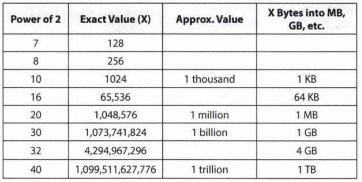
\includegraphics[width=10cm]{powers-of-two.png}
\end{figure}

\subsection{Array Sorting Algorithms Table}
\begin{figure}[h]
    \centering
    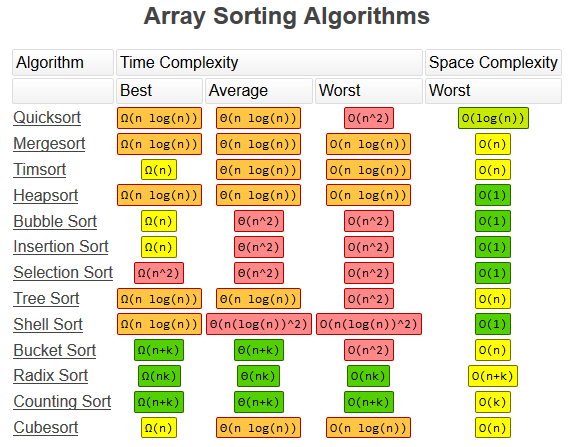
\includegraphics[width=13cm]{Array_sorting_algorithms.png}
\end{figure}

\subsection{Single-Source Shortest Path Table}
\begin{table}[H]
    \resizebox{\columnwidth}{!}{%
    % \centering
    \begin{tabular}{|l|l|l|l|l|}
        \hline
         Graph type & Algorithm & Time Complexity & Sparse $E=\bigO(V)$ & Dense $E=\bigO(V^2)$ \\
         \hline
         Unweighted & BFS & $\bigO(V + E)$ & $\bigO(V)$ & $\bigO(V^2)$  \\
         Positive Weights & Dijkstra & $\bigO(V \log V + E)$ & $\bigO(V \log V)$ & $\bigO(V^2)$\\
         General Weights & Bellman-Ford & $\bigO(V E)$ & $\bigO(V^2)$ & $\bigO(V^2)$ \\
         DAGs & Top. Sort + B-F & $\bigO(V + E)$  & $\bigO(V)$ & $\bigO(V^2)$ \\
         \hline
    \end{tabular}
    }
\end{table}


\subsection{Algorithm Optimization Checklist}
\begin{enumerate}
    \item Consider Best Conceivable Runtime (BCR). Try to derive an approach from an ideal upper bound on the solution.
    \item Consider making a time-space trade off, usually in the form of a hash-table or cached results.
    \item Data Structure Brainstorm. Linked List, Stack, Queue, Priority Queue, Heap, Dictionary, Set, Binary tree, Graph, etc.
    \item Simplify and Generalize. Simplify problem statement then attempt to generalize solution to original problem.
    \item Look for BUD (bottlenecks, unnecessary work, duplicated work).
    \item DIY (Do It Yourself). Design an algorithm around how you would solve an analogous real-word scenario without programming.
\end{enumerate}

\subsection{Whiteboard Interview Checklist}
\begin{enumerate}
    \item  Restate and reduce problem
    \begin{enumerate}
        \item Carefully read the problem. Spend some time simplifying and re-stating problem in your own words. This helps solidify your understanding, plus translating the problem into its most essential form may reveal possible reductions.
        \item Clarify requirements, constraints on input and any other assumptions you may need or want to make. 
        \item What are problematic or challenging areas that might arise from certain inputs? For example, an input that causes a naive approach to traverse the decision tree toward an incorrect solution. These inputs can be converted into sufficiently complex test cases later.
        \item Can you pre-process the input or re-interpret the desired output to simplify or reduce the problem to a simpler or familiar one? This may involve sorting a sequence, converting a matrix to a graph, etc.
        \item What is the best conceivable run time? If it's not yet obvious, this can be examined later during the optimization phase.
        \item What are your intuitions about possible solutions? You can revisit these ideas later.
    \end{enumerate}
    
    \item State brute-force solution
    \begin{enumerate}
        \item Give an overview of the approach.
        \item Find the time and space complexity.
        \item If you don't have any immediate ideas for an optimized solution, spend time elaborating on the brute force algorithm, otherwise mention that we can do better and can move on.
    \end{enumerate}
    
     \item Optimize previous approach or introduce new, better approach

    \begin{enumerate}
        \item Brainstorm using Algorithm Optimization Checklist. Avoid getting stuck on memory recall for too long, even you recognize the problem.
        \item Give an overview of the approach.
        \item Find the time and space complexity.
        \item Repeat or expand. Always spend extra time considering alternative approaches before implementing a solution.
        \item When out of ideas or if able to match the best conceivable run time with low/linear space complexity, prompt the interviewer for approval: ``If you're happy with this approach, I can go into the finer details and begin implemention''
    \end{enumerate}
    
     \item Consider more granular implementation details

    \begin{enumerate}
        \item Describe edge cases, i.e. empty input, invalid inputs, large inputs.
        \item Consider boundary conditions if dealing with iterations, indexed arrays, or ranges.
        \item Describe sufficiently complex test case if none are given, consider problem areas.
        \item Consider minor optimizations to general approach, i.e. short-circuiting, more performant data structures, caching.
        \item If using recursion, note the limitations of relying on the call stack. Default limit in Python is 1000.
    \end{enumerate}
    
    \item Implement
    \begin{enumerate}
        \item Speak aloud your thinking process, even when stuck.
        \item Handle base/empty cases, i.e. empty inputs, invalid input error checks.
        \item Use descriptive variable and function names.
        \item Add inline comments when necessary.
        \item Do not repeat yourself (DRY).
        \item Use modular code when possible.
        \item Follow coding principles (Correct, Efficient, Simple, Readable, Maintainable).
    \end{enumerate}
    
     \item Validate and test with dry runs
    \begin{enumerate}
        \item Scan over code and double check for any syntax errors.
        \item Walk through code using sufficiently complex test cases.
        \item Ensure boundary conditions don't cause errors.
        \item Clean up code if possible.
    \end{enumerate}
    
     \item Re-state final analysis
    \begin{enumerate}
        \item State time and space complexity of implementation.
        \item Consider further optimizations if time complexity is not BCR and space complexity is not constant.
    \end{enumerate}
\end{enumerate}

    
% \section{Notable Problems}
%     \subsection{Increment Sub-array}
    
%     \subsection{Find Duplicates with XOR}
    
%     \subsection{Peak Finding}
%     Binary search
    
%     \subsection{Document Distance}
%     1. split document into words
%     2. compute word frequencies
%     3. compute dot product

%     The "distance" between two vectors is the angle between them. If x = (x1, x2, ..., xn) is the first vector (xi = freq of word i) and y = (y1, y2, ..., yn) is the second vector, then the angle between them is defined as: d(x,y) = arccos(inner_product(x,y) / (norm(x)*norm(y))) where: inner_product(x,y) = x1*y1 + x2*y2 + ... xn*yn norm(x) = sqrt(inner_product(x,x))

\newpage
\begin{thebibliography}{}
\bibitem{a}
Steven S. Skiena. 2008. The Algorithm Design Manual (2nd. ed.). Springer Publishing Company, Incorporated.

\bibitem{b}
Erik Demaine, Srini Devadas. Introduction to Algorithms. Fall 2011. Massachusetts Institute of Technology: MIT OpenCouseWare, https://ocw.mit.edu/. License: Creative Commons

\bibitem{c}
David Liu, Data Structures and Analysis: Lecture Notes for CSC263, Department of Computer Science, University of Toronto

\bibitem{d}
McDowell, Gayle Laakmann, Cracking The Coding Interview: 150 Programming Questions and Solutions. Palo Alto, CA :CareerCup, LLC, 2011.

\bibitem{e}
Thomas H. Cormen, Charles E. Leiserson, Ronald L. Rivest, and Clifford Stein. 2009. Introduction to Algorithms, Third Edition (3rd. ed.). The MIT Press.


\bibitem{f}
Keller, M.T. and Trotter, W.T., Applied Combinatorics, Open Textbook Library,

ISBN9781534878655
\end{thebibliography}

\end{document}
